\documentclass[preprint,12pt]{elsarticle}

\usepackage{amsmath,amsfonts,amssymb}
\usepackage{algorithm}
\usepackage{algorithmic}
\usepackage{array}
\usepackage{subfig}
\usepackage{textcomp}
\usepackage{url}
\usepackage{graphicx}
\usepackage{booktabs}
\usepackage{makecell}
\usepackage{multirow}
\usepackage{adjustbox}
\usepackage{amsthm}
\usepackage[draft]{changes}

\definechangesauthor[
  name={Tingting Yang},
  color=red
]{R1}

\graphicspath{{figures/}{figures_en/}}

\journal{Future Generation Computer Systems-The International Journal of eScience}

\theoremstyle{plain}
\newtheorem{theorem}{Theorem}
\newtheorem{lemma}[theorem]{Lemma}
\newtheorem{proposition}[theorem]{Proposition}
\newtheorem{corollary}[theorem]{Corollary}
\newtheorem{assumption}[theorem]{Assumption}

\theoremstyle{definition}
\newtheorem{definition}[theorem]{Definition}

\theoremstyle{remark}
\newtheorem{remark}[theorem]{Remark}

\newcommand{\tabref}[1]{Table~\ref{#1}}
\newcommand{\figref}[1]{Fig.~\ref{#1}}
\newcommand{\secref}[1]{Section~\ref{#1}}
\newcommand{\equref}[1]{(\ref{#1})}
\newcommand{\method}{DynFedPrivacy}

\begin{document}

\begin{frontmatter}

\title{Dynamic Hierarchical Mode Selection for Cloud-Edge-End Federated Learning Under Resource Constraints and Privacy Protection}

\author[bupt]{Tingting Yang}
\author[bupt]{Wenbo Zhang}
\author[bupt]{Shaohua Liu}
\author[bupt]{Lihua Zhang}
\author[bupt]{Xinyuan Lin}
\author[bupt]{Qian Liu}

\affiliation[bupt]{organization={Beijing University of Posts and Telecommunications},
            city={Beijing},
            country={China}}

\begin{abstract}
Hierarchical federated learning (HFL) introduces edge nodes into federated learning so that IoT end devices can perform local training and edge nodes can conduct intermediate aggregation before cloud aggregation.
This structure reduces direct communication between IoT end devices and the cloud.
In practical IoT systems, end devices often have substantially different computation capabilities, memory capacities, and response delays.
Such device heterogeneity lowers training efficiency when delayed or weak devices are forced to follow the same training process as stronger devices.
Meanwhile, end devices, edge nodes, and cloud servers all operate under their own resource constraints.
Privacy requirements can further affect model accuracy because differential privacy (DP) noise may perturb model updates or intermediate representations.
This paper studies dynamic hierarchical mode selection for cloud-edge-end federated learning under resource constraints and privacy protection.


To address these challenges, we build a dynamic hierarchical mode selection method for cloud-edge-end federated learning.
We first analyze how DP perturbation and encrypted transmission overhead affect training efficiency and a convergence error proxy.
We then establish efficiency, privacy budget, and convergence error proxy models.
The proposed link graph representation describes different hierarchical training modes with Block units and Flow paths, which jointly capture computation, communication, aggregation, and privacy related interactions.
Based on this representation, we propose \method{}, a privacy aware dynamic hierarchical mode selection algorithm.
\method{} takes candidate hierarchical modes, link structures, and privacy mechanisms as input, and dynamically selects suitable model split positions and privacy mechanisms according to resource constraints, communication overhead, privacy budgets, and task requirements.
Experiments include Fashion-MNIST with LeNet-5 training and CIFAR-10 with ResNet-18 cloud-edge-end simulation.
Results show that \method{} can maintain resource and privacy feasibility, reduce the cost of fixed privacy mechanisms, and provide a tunable tradeoff among privacy consumption, training efficiency, and empirical test accuracy.
\end{abstract}

\begin{highlights}
\item A dynamic hierarchical mode selection problem is formulated for cloud-edge-end federated learning under resource and privacy constraints.
\item A Block and Flow based link graph represents computation, communication, aggregation, and privacy-related interactions across end, edge, and cloud layers.
\item DynFedPrivacy jointly considers latency, privacy budget, and convergence-error proxy when selecting hierarchical modes and privacy mechanisms.
\item Experiments on Fashion-MNIST/LeNet-5 and CIFAR-10/ResNet-18 show tunable tradeoffs among privacy consumption, training efficiency, and test accuracy.
\end{highlights}

\begin{keyword}
Internet of Things \sep hierarchical federated learning \sep cloud-edge-end collaboration \sep dynamic mode selection \sep differential privacy \sep device heterogeneity \sep resource constraints
\end{keyword}

\end{frontmatter}
\section{Introduction}
\label{sec:introduction}
Federated learning (FL) enables multiple end devices to collaboratively train a model by keeping data local and uploading only parameters or gradients~\cite{fedavg}.
With the development of artificial intelligence for IoT (AIoT), mobile edge computing, and intelligent sensing systems, training data are increasingly generated by cameras, mobile terminals, vehicles, and industrial sensors.
Cloud-edge-end hierarchical federated learning (HFL) has therefore been introduced to reduce long distance communication between end devices and the cloud through edge aggregation~\cite{hfl}.
It also enables multiple edge domains to participate in a shared cloud level training process.

However, HFL in cloud-edge-end environments still faces two major challenges.
First, end device data are usually non-IID, and significant distribution differences among devices can lead to model drift and performance degradation under simple weighted aggregation~\cite{fedavgm,fedprox}.
Second, IoT devices are system heterogeneous.
Low power cameras or sensors may be unable to support full training of a large deep model, whereas edge servers and cloud servers usually have stronger computation and memory resources~\cite{wang2019adaptivefl}.
If all devices are forced to follow the same training process, weak or delayed devices may become stragglers or may even be excluded by resource constraints.

Existing work has addressed these issues from several directions, but most studies improve a fixed HFL procedure rather than dynamically selecting how training tasks are assigned among the end, edge, and cloud layers.
Personalized HFL uses edge side personalization, similarity aware aggregation, or model decoupling to mitigate non-IID drift~\cite{Personalizedhfl,JSJX202502007}.
Resource constrained and wireless FL optimize local update frequency, communication rounds, energy consumption, or wireless resource allocation~\cite{wang2019adaptivefl,dinh2021wirelessfl}.
Cloud-edge-end collaborative HFL studies further consider heterogeneous model collaboration, multiple server edge aggregation, and split training mechanisms~\cite{BSBODP,mazloomi2025multiserver,SFETEC}.
Nevertheless, most existing methods are built around a specific collaborative procedure or a fixed hierarchical structure.
They pay insufficient attention to the mode selection variable, namely which model blocks should be executed at the end, edge, and cloud layers, which aggregation flow should be used, and how this task assignment should interact with privacy mechanisms.

Privacy protection further complicates this decision.
DP limits the influence of a single sample or client by clipping and perturbing features or updates, but it may degrade convergence.
Adaptive DP methods tune privacy budgets, clipping thresholds, and client selection to improve the privacy utility tradeoff~\cite{GLDP,xu2025adpfl,elabd2025dynamicdp}.
HE, secure aggregation, and privacy preserving offloading have also been studied in FL and cloud-edge-end systems~\cite{dong2026privacyoffloading,PPHFL,islam2025pphffl}.
Different hierarchical modes expose different privacy related objects.
For example, split training between end devices and edge nodes may transmit intermediate features, whereas aggregation between edge nodes and the cloud mainly transmits gradients or model updates.
Therefore, the communication, computation, and convergence error effects of privacy mechanisms should be modeled together with hierarchical mode selection.

This paper studies dynamic hierarchical mode selection for cloud-edge-end federated learning under resource constraints and privacy protection.
In this paper, dynamic hierarchy is realized through mode selection: each mode specifies how model computation and aggregation are assigned among the end, edge, and cloud layers.
The main contributions are as follows:
\begin{itemize}
    \item We formulate dynamic hierarchical mode selection for cloud-edge-end FL, where training tasks can be assigned to end devices, edge nodes, and the cloud according to device heterogeneity, resource constraints, communication overhead, and privacy requirements.
    \item We define a Block and Flow based link graph to represent hierarchical training modes. This representation describes model block execution, cross layer transmission, aggregation, model return, and privacy related interactions in a unified form.
    \item We establish a joint cost model for latency, communication, privacy budget, and a convergence error proxy. The model captures the effects of DP perturbation, encrypted transmission overhead, synchronization waiting, and cloud level fusion.
    \item We develop \method{}, a privacy aware mode selection algorithm that searches feasible hierarchical modes and privacy mechanism assignments under resource and privacy constraints.
    \item We evaluate \method{} using Fashion-MNIST/LeNet-5 training and CIFAR-10/ResNet-18 experiments, including data distribution, resource heterogeneity, strategy update period, aggregation fraction, and multiple random seed analyses.
\end{itemize}

\section{Related Work}
\label{sec:related_work}
\subsection{HFL Under Heterogeneous Environments}
HFL introduces edge servers between end devices and the cloud to reduce direct cloud communication pressure through edge pre aggregation~\cite{hfl}.
Resource aware FL studies reduce stragglers and communication overhead by adjusting client selection, local update frequency, pruning, or model compression under limited computation, energy, and bandwidth resources~\cite{phfl,xu2022adaptive,wang2019adaptivefl,dinh2021wirelessfl}.
Personalized HFL further mitigates performance degradation under non-IID data through edge side personalized models, similarity aggregation, or model decoupling~\cite{Personalizedhfl,JSJX202502007}.
These methods show that HFL can improve training from resource scheduling, communication control, and data heterogeneity adaptation.
However, when end device resources differ across computation, memory, and communication capabilities, using the same training flow for all clients can still slow synchronous aggregation and block weak devices.
This paper jointly considers end device computation constraints, memory constraints, communication overhead, and model split positions during mode selection.
\added[id=R1]{Dynamic selection itself may also introduce reconfiguration overhead. Recent multi-job FL studies explicitly model switching cost in client selection and reduce it through block-wise selection, where the selected client subset is kept unchanged across multiple rounds rather than being changed every round~\cite{CHEN2026112204,10757319}. This observation motivates the use of a strategy update period in our framework: hierarchical modes are re-evaluated only at update points, which limits unnecessary mode reconfiguration while preserving adaptability to resource and link changes.}

\subsection{Cloud-Edge-End Collaborative Federated Learning}
HFL is a representative form of cloud-edge-end collaborative FL, in which end devices, edge nodes, and the cloud jointly execute computation, aggregation, and communication tasks.
As model size and system heterogeneity increase, fixed full end device training followed by edge aggregation becomes less suitable for resource limited IoT devices.
FedAgg~\cite{BSBODP} uses bridge samples and online distillation to enable models of different scales at the end, edge, and cloud layers to collaborate.
SFETEC~\cite{SFETEC} introduces split federated learning into Thing Edge Cloud environments and partitions model computation across layers to reduce end device computation load.
Cloud-edge-end task offloading studies also combine FL, privacy protection, and task efficiency~\cite{dong2026privacyoffloading}.
These studies show the value of collaboration among the three layers, but they usually assume a fixed mode selection strategy.
In contrast, this paper studies how each device should select a hierarchical training mode under given resource and privacy conditions.
\added[id=R1]{The need to balance reconfiguration gain and reconfiguration cost is also consistent with edge-computing task migration studies. In mobile edge computing, migration can reduce service delay when users move away from the original edge server, but it also consumes backhaul transmission and reconfiguration resources~\cite{ZHANG2019111}. Load-aware task migration further models migration cost as a combination of communication, queuing, and computation costs, and notes that migration cost can be related to physical distance between edge nodes~\cite{ZHU2024303}. These studies suggest that dynamic cloud-edge-end collaboration should account for both the benefit of changing execution paths and the overhead caused by such changes.}

\subsection{Privacy Preserving HFL}
Model parameters, gradients, and intermediate representations in federated training may leak information about private data.
Differential privacy (DP), homomorphic encryption (HE), and secure aggregation are therefore widely used in FL.
For HFL, group local DP provides personalized privacy through sampling, randomized response, and shuffling~\cite{GLDP}.
Adaptive DP-FL improves convergence and model utility through dynamic privacy budget allocation, adaptive clipping, and client selection~\cite{xu2025adpfl}.
Other privacy preserving HFL studies combine client level DP, secure aggregation, and CKKS-style HE for data space scenarios~\cite{PPHFL}, or combine hierarchical fog FL, personalization, and DP for IoT intrusion detection~\cite{islam2025pphffl}.
These studies mainly focus on the security guarantee, budget allocation, or accuracy degradation of a particular privacy mechanism.
The joint modeling of privacy induced communication cost, computation latency, convergence error proxy, and cloud-edge-end mode selection remains insufficiently studied.

\section{Model Construction}
\label{sec:model}
\subsection{Cloud-Edge-End Collaborative Link Modeling}
\label{sec:link_model}
We consider a three tier cloud-edge-end collaborative FL system composed of end devices, edge nodes, and a cloud node.
Let \(\mathcal{N}\) denote the set of end devices.
Each end device \(i\in\mathcal{N}\) selects one hierarchical mode \(h_i\) from a candidate mode set \(\mathcal{H}\).
In this paper, a hierarchical mode specifies the model split position, the layer that executes each model block, and the return path of aggregation results.
Given a global model \(M\), different modes correspond to different model partitions:
\begin{equation}
    M = M_L^{h_i} \cup M_E^{h_i} \cup M_C^{h_i},
\end{equation}
where \(M_L^{h_i}\), \(M_E^{h_i}\), and \(M_C^{h_i}\) are the submodels executed at the end, edge, and cloud layers, respectively.
Weaker devices use split positions closer to the input layer and offload more computation to the edge or cloud, whereas stronger devices can undertake a larger proportion of local training.

\begin{definition}[Block]
Given a cloud-edge-end mode \(h_i\), a Block is the local training step and cross layer interaction associated with end device \(i\) before an aggregation event.
Formally,
\begin{equation}
    B_i^{h_i}=(d_i,\ell_i,g_i,\mathcal{E}_{B,i}^{h_i}),
\end{equation}
where \(d_i\) is the participating end device, \(\ell_i\in\{L,E,C\}\) indicates the layer that stores or updates the local trainable parameters, \(g_i\in\{A_e,A_c\}\) is the aggregation node that receives the update, and \(\mathcal{E}_{B,i}^{h_i}\) is the set of intermediate feature, gradient, or update transmission links caused by split training.
According to the execution layer \(\ell_i\), we denote the corresponding Block as \(B_L\), \(B_E\), or \(B_C\), which means that the trainable part of the model is executed at the end, edge, or cloud layer, respectively.
\end{definition}

\begin{definition}[Flow]
A Flow is a complete training link formed by one or more Blocks, the aggregation node, and the model return process.
A one level aggregation Flow can be abstracted as
\begin{equation}
    \text{Flow}: d_i \xrightarrow{B_i^{h_i}\times L_B} \ell_i
    \xrightarrow{\text{upload}} a
    \xrightarrow{\text{download}} q_i .
\end{equation}
Here, \(\xrightarrow{B_i^{h_i}\times L_B}\) denotes that end device \(i\) performs \(L_B\) Blocks under hierarchical mode \(h_i\), with the resulting training process terminating at layer \(\ell_i\). \(a\) is the selected aggregation node, and \(q_i\) is the node that receives the returned model or submodel for device \(i\).
If two level aggregation exists, the Flow also contains an edge aggregation node \(A_e\), the cloud aggregation node \(A_c\), and the final return to the end device:
\begin{equation}
\begin{aligned}
    \text{Flow}: [d_i \xrightarrow{B_i^{h_i}\times L_B} \ell_i
    \xrightarrow{\text{upload}} A_e] \times E_B\\
    \xrightarrow{\text{upload}} A_c
    \xrightarrow{\text{download}} A_e
    \xrightarrow{\text{download}} d_i .
\end{aligned}
\end{equation}
\end{definition}

\begin{definition}[Cloud-Edge-End Collaborative Link Graph]
For a hierarchical mode \(h_i\), its training process is represented by a directed link graph
\begin{equation}
    \mathcal{G}^{h_i}=(\mathcal{V},\mathcal{E}),
\end{equation}
where \(\mathcal{V}\) contains end, edge, and cloud nodes, and
\(\mathcal{E}\) contains the interaction links among them.
\replaced[id=R1]{Each interaction link is defined as}{Each interaction link is defined as}
\begin{equation}
    \replaced[id=R1]{\lambda=(u,v,b,P_{\lambda},S_{\lambda},R_{u,v},T_{\lambda})}{e=(u,v,b,P_e,S_e,R_{u,v},T_e)},
\end{equation}
where \(u\) and \(v\) are the source and target nodes, \(b\) is the interaction type,
\replaced[id=R1]{\(P_{\lambda}\) is the privacy mechanism, \(S_{\lambda}\) is the processed transmission size, \(R_{u,v}\) is the link rate, and \(T_{\lambda}\) is the induced latency.}{\(P_e\) is the privacy mechanism, \(S_e\) is the processed transmission size, \(R_{u,v}\) is the link rate, and \(T_e\) is the induced latency.}
\end{definition}

\begin{figure}[t]
\centering
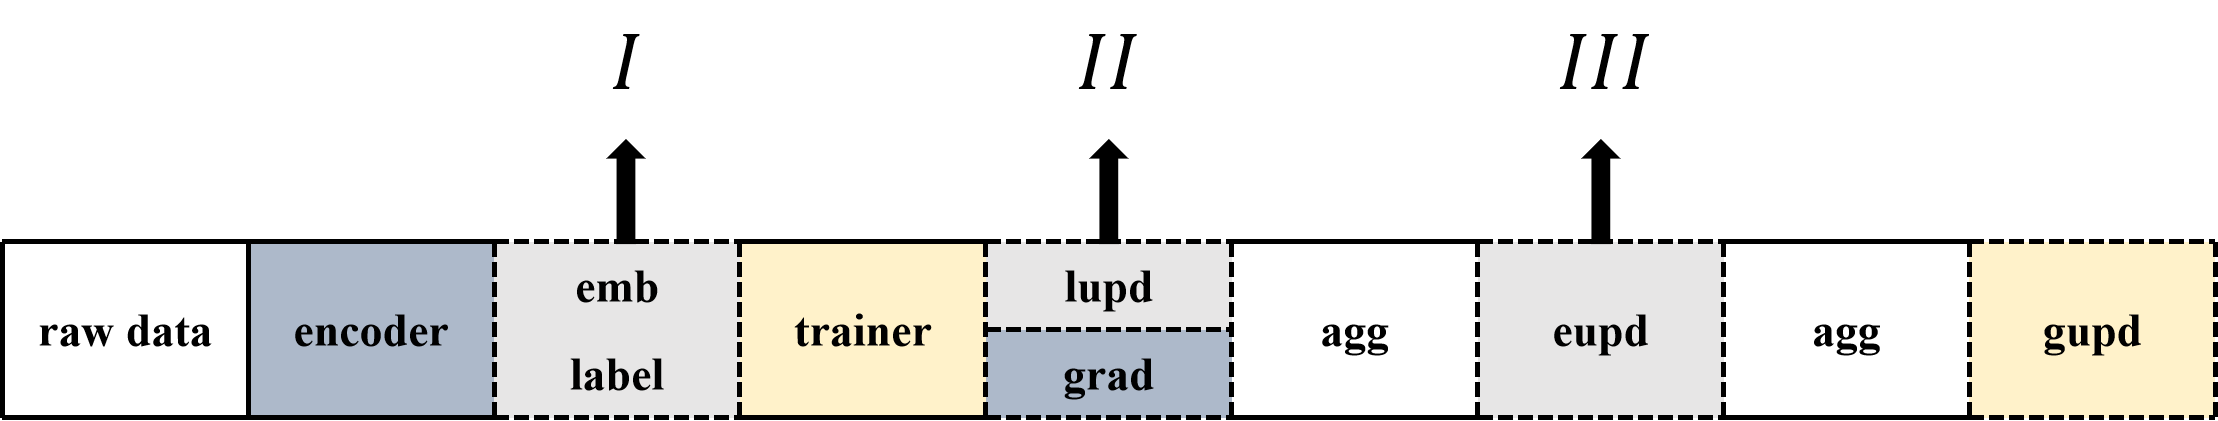
\includegraphics[width=\columnwidth]{classic.png}
\caption{\replaced[id=R1]{Abstract training flow and candidate split interfaces in cloud-edge-end collaborative FL. From left to right, raw data are processed by the encoder, while the label is kept on the data owner side as supervision. The intermediate embedding \(\mathrm{emb}\) can be transmitted across interface I to the trainer. The local update \(\mathrm{lupd}\) and backward gradient \(\mathrm{grad}\) describe the local optimization and split backward propagation stage around interface II. The two aggregation blocks represent edge level and cloud level aggregation, respectively; \(\mathrm{eupd}\) and \(\mathrm{gupd}\) denote edge update and global update transmissions around interface III and after cloud aggregation. Interfaces I, II, and III mark candidate interaction boundaries from shallow to deep stages rather than ordinary neural network layers. Moving the split interface deeper keeps more computation on the end side, while moving it earlier offloads more computation to the edge or cloud side.}{Classical federated learning process and model split interfaces. The end device first executes the front part of the model on local data, the intermediate computation result or model update is then transmitted to the edge or cloud side, and the aggregated model is returned for the next round. Interfaces I, II, and III mark candidate partition points from shallow to deep layers; moving the split interface deeper means that more model computation remains at the end side, whereas moving it earlier offloads more computation to the edge or cloud side.}}
\label{fig:classic}
\end{figure}

\replaced[id=R1]{Based on the abstract training flow and candidate interaction boundaries illustrated in \figref{fig:classic}, for the three layer structure composed of end (\(L\)), edge (\(E\)), and cloud (\(C\)), this paper considers seven basic modes. In the figure, interface I corresponds to feature level transmission, interface II corresponds to local update and backward gradient interaction in split training, and interface III corresponds to edge or global update transmission across aggregation stages.}{Based on the model split interfaces illustrated in \figref{fig:classic}\comment[id=R1]{The explanation of this picture isn't good either; it doesn't explain what the different parts of the picture mean.}, for the three layer structure composed of end (\(L\)), edge (\(E\)), and cloud (\(C\)), this paper considers seven basic modes:}
\begin{equation}
\mathcal{H}=\{\mathrm{LIE},\mathrm{LIC},\mathrm{LIIE},\mathrm{LIIC},\mathrm{LIEIIC},\mathrm{LIEIIIC},\mathrm{LIIEIIIC}\}.
\end{equation}
The symbols \(L\), \(E\), and \(C\) indicate the layer that executes or stores the trainable model block, while \(\mathrm{I}\), \(\mathrm{II}\), and \(\mathrm{III}\) denote the selected model split interface.

\begin{definition}[Block Transmission Indicator Matrix]
Let the node order be \((L,E,C)\), and let \replaced[id=R1]{\(\mathcal{B}=\{\mathrm{emb},\mathrm{grad},\mathrm{upd}\}\)}{\(\mathcal{B}=\{\mathrm{emb},\mathrm{upd}\}\)}\comment[id=R1]{It doesn't explain what the letters "emb" and "upd" mean.}, where \(\mathrm{emb}\) abbreviates embedding or intermediate feature transmission, \added[id=R1]{\(\mathrm{grad}\) denotes backward gradient transmission in split training,} and \replaced[id=R1]{\(\mathrm{upd}\) denotes model update or aggregation result transmission}{\(\mathrm{upd}\) abbreviates model update or aggregation result transmission}.
For mode \(h_i\) and transmission type \(b\in\mathcal{B}\), the Block transmission indicator matrix is
\begin{equation}
    \mathbf{I}_{b}^{h_i}(u,v)=
    \begin{cases}
    1, & \text{mode } h_i \text{ transmits type } b \text{ from } u \text{ to } v,\\
    0, & \text{otherwise}.
    \end{cases}
\end{equation}
For example, for LIEIIC,
\begin{equation}
\mathbf{I}_{\mathrm{emb}}^{\mathrm{LIEIIC}}=
\begin{pmatrix}
0 & 1 & 0\\
0 & 0 & 0\\
0 & 0 & 0
\end{pmatrix}.
\end{equation}
\end{definition}

Different transmission types admit different privacy mechanisms.
Intermediate features \added[id=R1]{and backward gradients} are directly related to sample representations \added[id=R1]{and training signals}, so this paper allows DP perturbation for them.
Model updates can use DP perturbation or HE transmission~\cite{PPHFL}.\comment[id=R1]{I can add a citation here}
The candidate privacy mechanism assignment set under mode \(h_i\) is denoted by \(\Pi(h_i)\), and \(\mathcal{P}_i\in\Pi(h_i)\) specifies whether each privacy sensitive transmission type is protected by DP or by HE.
In other words, for a protected training policy, a transmission link that does not use DP is assumed to use HE, while the no protection case is used only as an experimental baseline.

\textbf{Flow representation of seven hierarchical modes.}
Let \(A_e\) and \(A_c\) denote the edge and cloud aggregators, respectively.
Let \(L_B\) be the number of local Block loops, and let \(E_B\) be the number of edge aggregation loops before cloud aggregation.
Here \(L_B\) and \(E_B\) denote loop counts, which avoids confusion with the end layer \(L\) and the edge layer \(E\).
The notation \(\xrightarrow{0}\) indicates no cross node transmission, and \(\xrightarrow{1}\) indicates cross node transmission that may require a privacy mechanism.
\begin{itemize}
    \item \textbf{LIE:} \(\mathcal{F}(\mathrm{LIE}) = B_E \times L_B \xrightarrow{0} A_e \xrightarrow{1} \mathrm{end}\).
    \item \textbf{LIIE:} \(\mathcal{F}(\mathrm{LIIE}) = B_L \times L_B \xrightarrow{1} A_e \xrightarrow{1} \mathrm{end}\).
    \item \textbf{LIC:} \(\mathcal{F}(\mathrm{LIC}) = B_C \times L_B \xrightarrow{0} A_c \xrightarrow{1} \mathrm{end}\).
    \item \textbf{LIIC:} \(\mathcal{F}(\mathrm{LIIC}) = B_L \times L_B \xrightarrow{1} A_c \xrightarrow{1} \mathrm{end}\).
    \item \textbf{LIEIIC:} \(\mathcal{F}(\mathrm{LIEIIC}) = B_E \times L_B \xrightarrow{1} A_c \xrightarrow{1} A_e \xrightarrow{1} \mathrm{end}\).
    \item \textbf{LIEIIIC:} \(\mathcal{F}(\mathrm{LIEIIIC}) = [B_E \times L_B \xrightarrow{0} A_e \xrightarrow{1} \mathrm{end}] \times E_B \xrightarrow{1} A_c \xrightarrow{1} A_e \xrightarrow{1} \mathrm{end}\).
    \item \textbf{LIIEIIIC:} \(\mathcal{F}(\mathrm{LIIEIIIC}) = [B_L \times L_B \xrightarrow{1} A_e \xrightarrow{1} \mathrm{end}] \times E_B \xrightarrow{1} A_c \xrightarrow{1} A_e \xrightarrow{1} \mathrm{end}\).
\end{itemize}
The corresponding cloud-edge-end collaborative link graphs of the seven modes are illustrated in \figref{fig:eecblockflow}.\comment[id=R1]{It doesn't give the details of the image. I need to describe these images meticulously.} In the figure, each row corresponds to one mode, the end, edge, and cloud columns indicate where model blocks are executed or stored, solid cross layer arrows denote actual transmission, and zero marked transitions denote local aggregation or local state update without cross node communication. Modes LIE and LIIE finish aggregation at the edge side, LIC and LIIC directly involve the cloud side, LIEIIC introduces cloud aggregation after edge side block execution, and LIEIIIC and LIIEIIIC add repeated edge side aggregation loops before cloud level aggregation and model return.
\begin{figure*}[t]
\centering
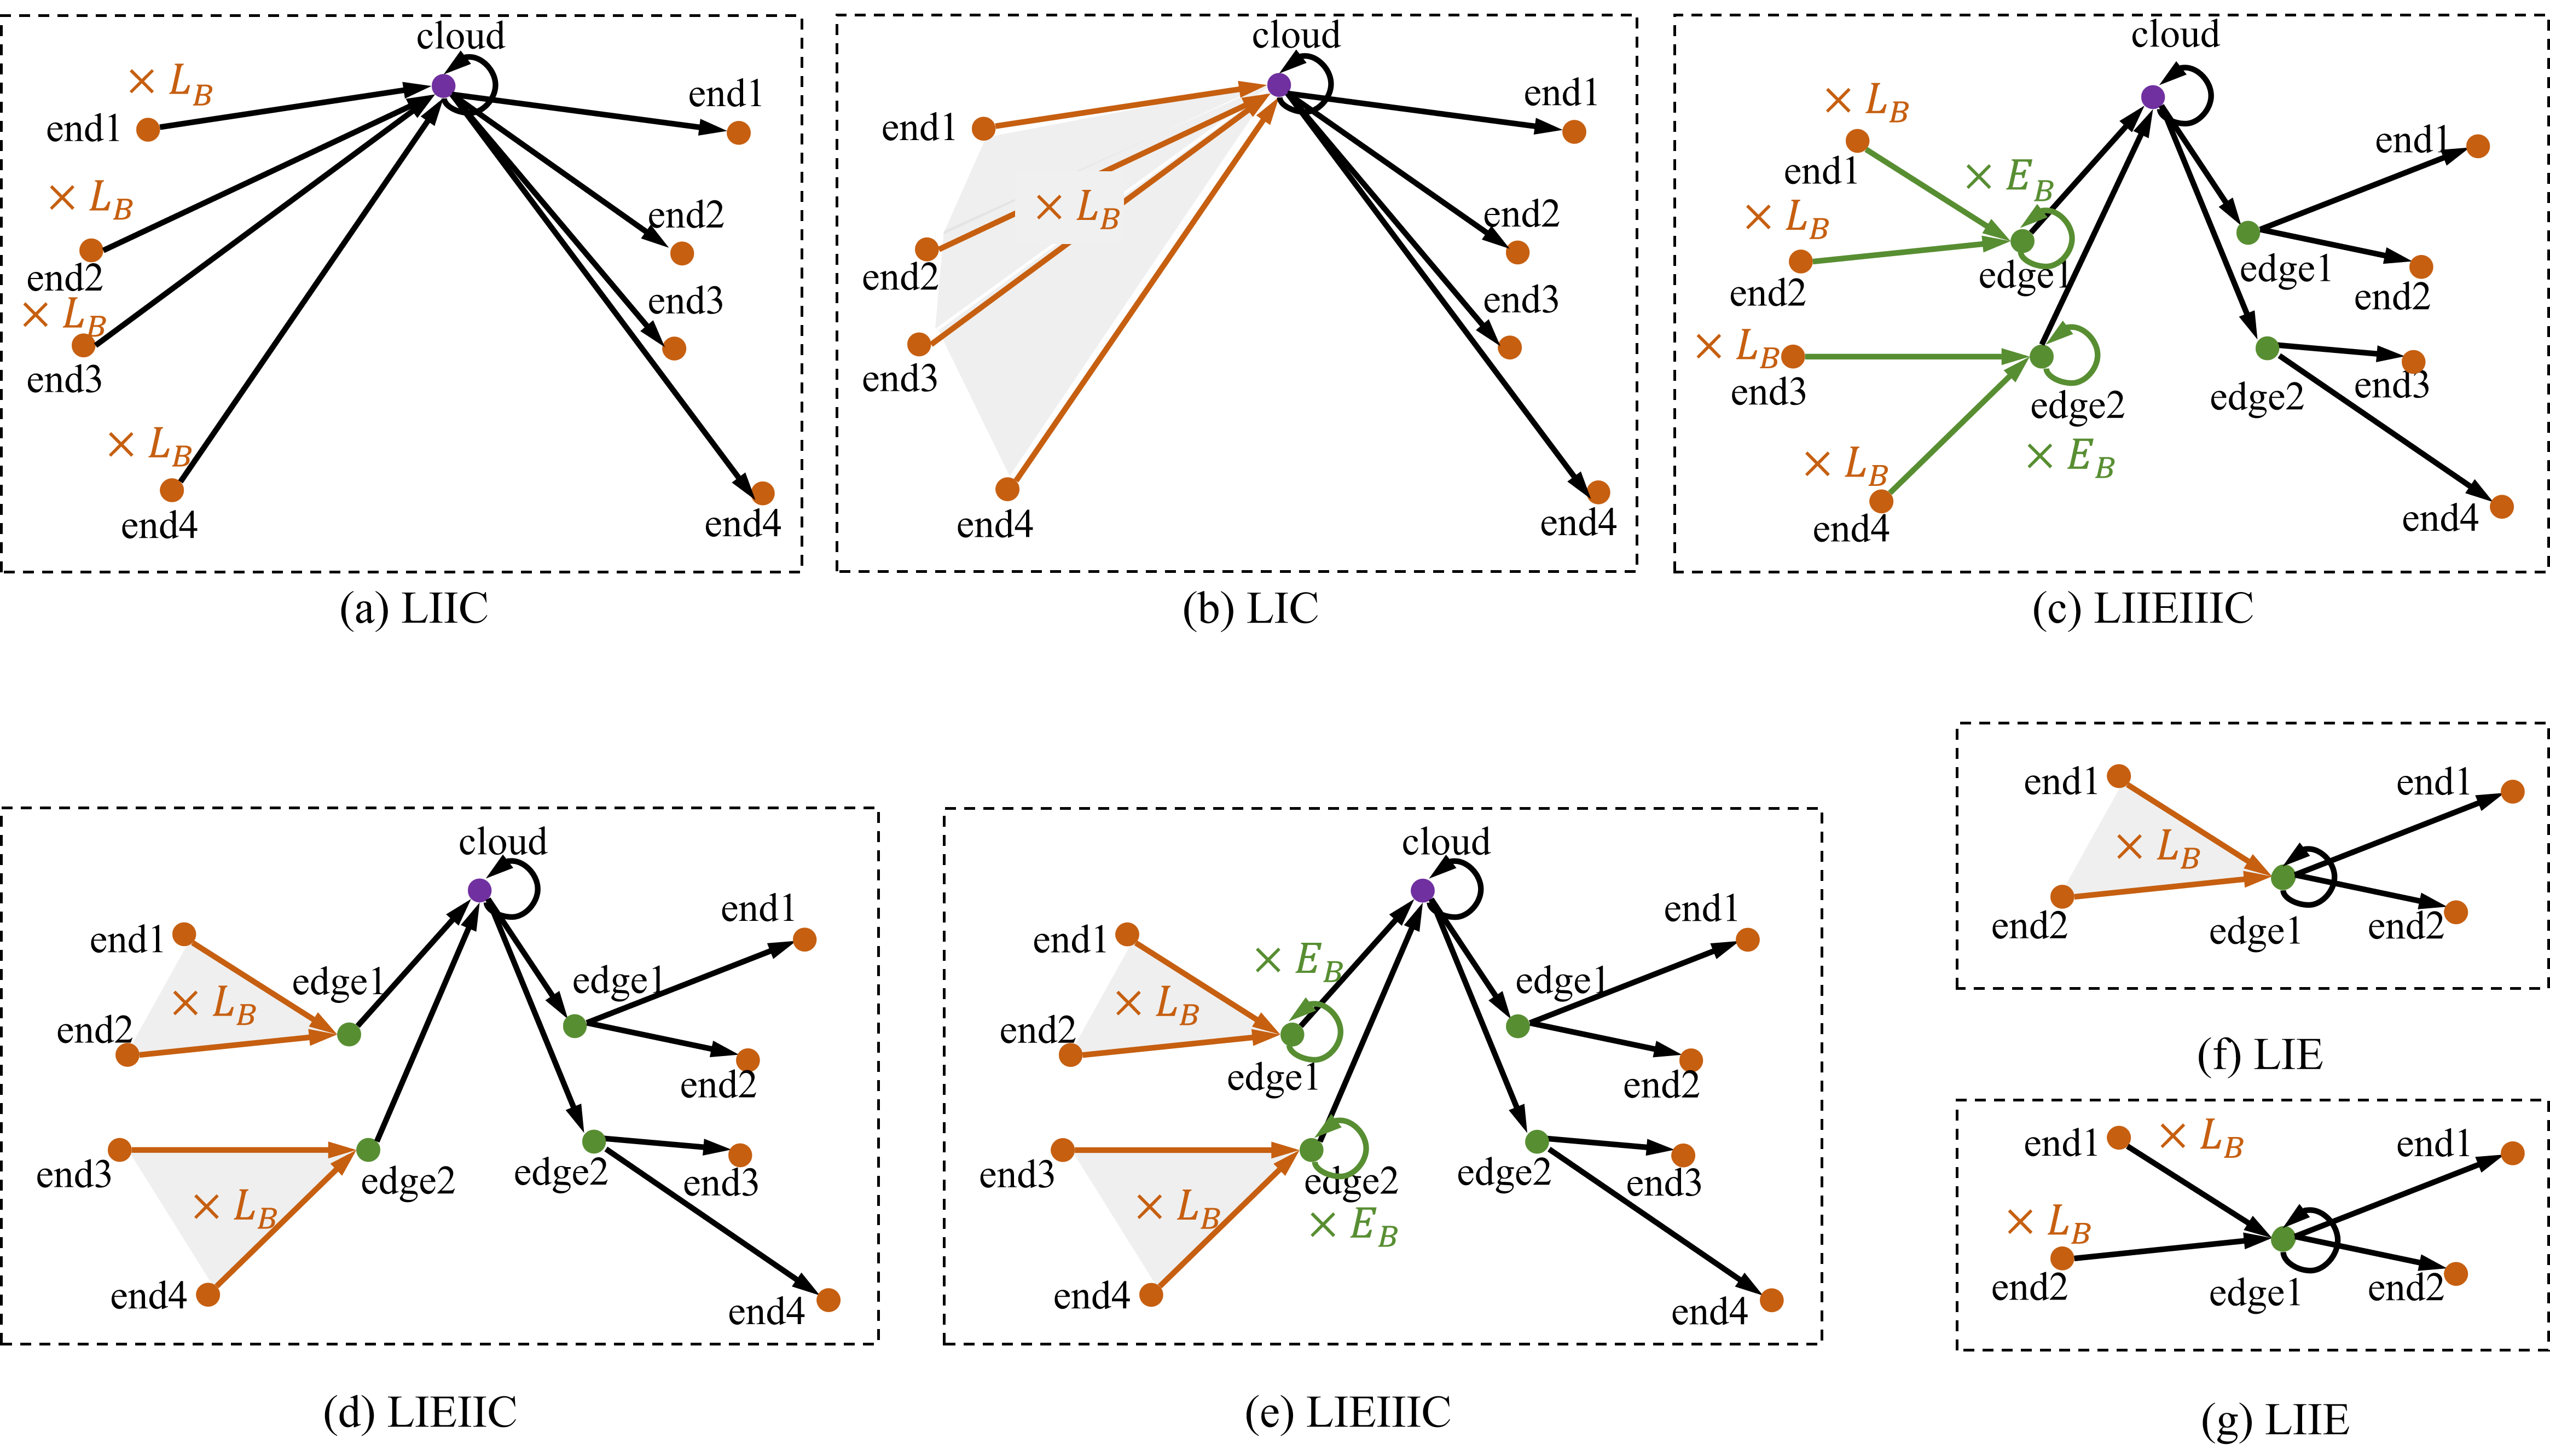
\includegraphics[width=\textwidth]{eecblockflow.png}
\caption{Cloud-edge-end collaborative link graphs of the seven hierarchical modes.}
\label{fig:eecblockflow}
\end{figure*}

\subsection{Joint Cost and Utility Modeling}
\label{sec:cost_utility_model}
\highlight[id=R1]{After the link topology is determined}, each decision pair \((h_i,\mathcal{P}_i)\) must satisfy end side resource feasibility and balance training efficiency, privacy budget consumption, and convergence error proxy.
The end side computation cost \(C_i^{\mathrm{comp}}\) and memory cost \(C_i^{\mathrm{mem}}\) are defined as follows.
Let \(m_i(h_i)\) be the parameter scale undertaken by end device \(i\) under mode \(h_i\), \(a_i(h_i)\) be the activation and gradient cache size, and \(n_i\) be the local per round sample count.
The single round local computation cost is
\begin{equation}
    C_i^{\mathrm{comp}}(h_i,n_i,m_i)=\gamma L_B n_i m_i(h_i),
\end{equation}
\comment[id=R1]{I need a citation to explain why it's a linear relationship.}
where \(\gamma\) is a normalized coefficient reflecting the computation intensity of the adopted model architecture. The linear proxy follows the common estimation that local training work scales with the number of processed samples, local update loops, and the parameter scale executed on the device~\cite{fedavg,wang2019adaptivefl}.
The end side memory cost is
\begin{equation}
    C_i^{\mathrm{mem}}(h_i)=\kappa_m m_i(h_i)+\kappa_a a_i(h_i).
\end{equation}
Here, \(\kappa_m\) and \(\kappa_a\) are normalized coefficients representing the relative memory overhead of model parameters and intermediate feature/gradient cache, respectively. Their values are set according to the normalized memory requirement of the adopted model architecture.

Let \(Q_{c,i}\) and \(Q_{e,i}\) be the computation and memory budgets of device \(i\).
The resource feasible mode set is
\begin{equation}
    \mathcal{H}_i=
    \{h_i\in\mathcal{H}\mid
    C_i^{\mathrm{comp}}(h_i,n_i,m_i)\le Q_{c,i},
    C_i^{\mathrm{mem}}(h_i)\le Q_{e,i}\}.
\label{eq:resource_feasible}
\end{equation}

Let \(R^t=(R_{u,v}^t)_{u,v\in\mathcal{V}}\) be the cloud-edge-end link rate matrix in round \(t\).
\added[id=R1]{The communication model is link specific. For an end-edge pair \((i,j)\), the rate \(R_{i,j}^{t}\) and the base latency \(T_{i,j}^{0}\) may differ from those of other device-edge pairs. These parameters capture heterogeneous physical distance, wireless channel quality, interference, and congestion, so two end devices connected to the same edge server, or the same device connected to different edge servers, may have different communication latency~\cite{ZHANG2019111,ZHU2024303}.}
\replaced[id=R1]{For an interaction link \(\lambda=(u,v,b)\), its raw transmission size is \(S_{\lambda}^t(h_i,b)\).}{For an interaction link \(\lambda=(u,v,b)\), its raw transmission size is \(S_{\lambda}^t(h_i,b)\).}
After privacy processing, the effective transmission size is \(\alpha(\mathcal{P}_i(b))\replaced[id=R1]{S_{\lambda}^t(h_i,b)}{S_e^t(h_i,b)}\), where \(\alpha(\cdot)\) is the communication inflation factor induced by the selected privacy mechanism.\comment[id=R1]{Maybe alpha here should mean the communication inflation factor.}
For DP, \(\alpha(\mathrm{DP})\approx 1\); for HE, ciphertext encoding and encrypted processing increase the transmitted size, so \(\alpha(\mathrm{HE})>1\)~\cite{PPHFL}.\comment[id=R1]{Why are there two citations?}
The communication latency is
\begin{equation}
T_{u,v}^{\mathrm{comm},t}(h_i,b,\mathcal{P}_i)
=
\frac{\alpha(\mathcal{P}_i(b))
\replaced[id=R1]{S_{\lambda}^t(h_i,b)}{S_e^t(h_i,b)}}
{R_{u,v}^{t}}
+T_{u,v}^{0}+T_{u,v}^{P}(\mathcal{P}_i(b)),
\label{eq:comm_latency}
\end{equation}
where \(T_{u,v}^{0}\) is the base link latency\comment[id=R1]{I think this symbol should have only one meaning, not two. Select from ink latency or random perturbation.}, and \(T_{u,v}^{P}\) is additional privacy processing latency. Round level network fluctuation is represented by the time varying link rate \(R_{u,v}^{t}\).

\replaced[id=R1]{The path level Flow latency of end device \(i\), denoted by \(T_i(h_i,\mathcal{P}_i)\), is decomposed into computation, communication, waiting, and aggregation components.}{The Flow latency of end device \(i\) is further expanded by considering the specific computation, communication, waiting, and aggregation processes along the cloud-edge-end path.}
\comment[id=R1]{The compact path-level latency \(T_i(h_i,\mathcal{P}_i)\) is needed because it is later used in \(T_{\mathrm{sys}}\). Fig.~\ref{fig:time} and the following expanded expression should explain where the compact components come from, rather than introduce \(T_i^{\mathrm{total}}\) as a separate variable.}
\added[id=R1]{Let \(\mathcal{E}_{\mathrm{flow}}^{h_i}\) be the set of cross node interaction links that occur in one complete Flow under mode \(h_i\), and let \(N_{\lambda}(h_i)\) be the number of times link \(\lambda\) is executed.}
\added[id=R1]{The compact path level latency model is}
\begin{equation}
\begin{aligned}
T_i(h_i,\mathcal{P}_i)
&=T_i^{\mathrm{comp}}(h_i)
+\sum_{\lambda\in\mathcal{E}_{\mathrm{flow}}^{h_i}}
N_{\lambda}(h_i)T_{\lambda}^{\mathrm{comm},t}\\
&\quad +T_i^{\mathrm{wait}}(h_i)
+T_i^{\mathrm{agg}}(h_i,\mathcal{P}_i)
\added[id=R1]{+C_i^{\mathrm{sw},t}}.
\end{aligned}
\label{eq:latency_model}
\end{equation}
\added[id=R1]{Here, \(T_i^{\mathrm{comp}}\) denotes the computation latency of the submodels executed along the Flow, \(T_i^{\mathrm{wait}}\) denotes the waiting latency before edge or cloud aggregation is triggered, and \(T_i^{\mathrm{agg}}\) denotes the aggregation and privacy processing latency assigned to the Flow.}
\added[id=R1]{The optional term \(C_i^{\mathrm{sw},t}\) denotes mode reconfiguration overhead in round \(t\). It can represent model-block redistribution, cached state synchronization, aggregation-path reconfiguration, and privacy-mechanism setup when the current decision differs from the previous decision. A simple instance is}
\begin{equation}
\added[id=R1]{
C_i^{\mathrm{sw},t}
=\eta_h \mathbb{I}(h_i^t\neq h_i^{t-1})
+\eta_p \mathbb{I}(\mathcal{P}_i^t\neq \mathcal{P}_i^{t-1})
+\eta_s D(h_i^t,h_i^{t-1}),
}
\label{eq:switching_cost}
\end{equation}
\added[id=R1]{where \(\eta_h\), \(\eta_p\), and \(\eta_s\) are nonnegative coefficients for mode switching, privacy-mechanism switching, and structural model-partition changes, respectively. The distance \(D(h_i^t,h_i^{t-1})\) measures the difference between two hierarchical modes, such as changes in split interfaces, migrated model blocks, or modified transmission paths. If real deployment measurements are unavailable, this term can be set to zero and the reconfiguration frequency can instead be controlled through the strategy update period.}
To mitigate synchronization blocking caused by slow devices, we use an asynchronous buffered aggregation mechanism.
For edge aggregator \(j\), let \(N_j\) be the number of associated end devices and \(\rho_{\mathrm{buf}}\in(0,1]\) be the buffered aggregation participation threshold.
The number of clients needed to trigger aggregation is \(K_j=\lceil\rho_{\mathrm{buf}} N_j\rceil\).
Let \(T_i^{\mathrm{lupd}}\) be the time needed for device \(i\) to complete local or collaborative update.
The arrival time at edge \(j\) is
\begin{equation}
x_{i,j}^t=T_i^{\mathrm{lupd}}(h_i,\mathcal{P}_i)+T_{i,j}^{\mathrm{comm},t}(h_i,\mathcal{P}_i).
\end{equation}
Sorting arrival times as \(x_{(1),j}^t\le\cdots\le x_{(N_j),j}^t\), the edge aggregation start time and waiting time are
\begin{equation}
X_j^t=x_{(K_j),j}^t,\quad
W_{i,j}^{\mathrm{agg},t}=\max(0,X_j^t - x_{i,j}^t).
\end{equation}
The edge aggregation time is
\begin{equation}
T_j^{\mathrm{agg},t}=\beta_j |S_j^t|S_{\mathrm{agg}}^t+T_j^{\mathrm{fix}}+T_j^{P,t}.
\end{equation}
where \(\beta_j\) is the aggregation processing coefficient of edge aggregator \(j\), \(S_j^t\) denotes the set of client updates selected into the buffered aggregation at edge aggregator \(j\) in round \(t\), and \(\lvert S_j^t\rvert\) represents the number of selected updates actually involved in aggregation. Under exact threshold triggering, \(\lvert S_j^t\rvert=K_j\); if the implementation admits all updates that have arrived by the trigger instant, then \(\lvert S_j^t\rvert\ge K_j\).

\(S_{\mathrm{agg}}^t\) represents the equivalent data size of one selected client update in aggregation computation, measured by the model update vector size, parameter dimension, or privacy processed aggregation payload.\comment[id=R1]{I think this description is not clear. Maybe the reader cannot understand the meaning of the symbol Saggt.}
\(T_j^{\mathrm{fix}}\) denotes the fixed aggregation overhead independent of the number and size of updates, and \(T_j^{P,t}\) denotes the additional latency caused by privacy processing at edge aggregator \(j\) in round \(t\).\comment[id=R1]{Maybe we need to add an explanation of how to obtain the value for the Tjagg. equation or citation.}
\begin{figure}[t]
\centering
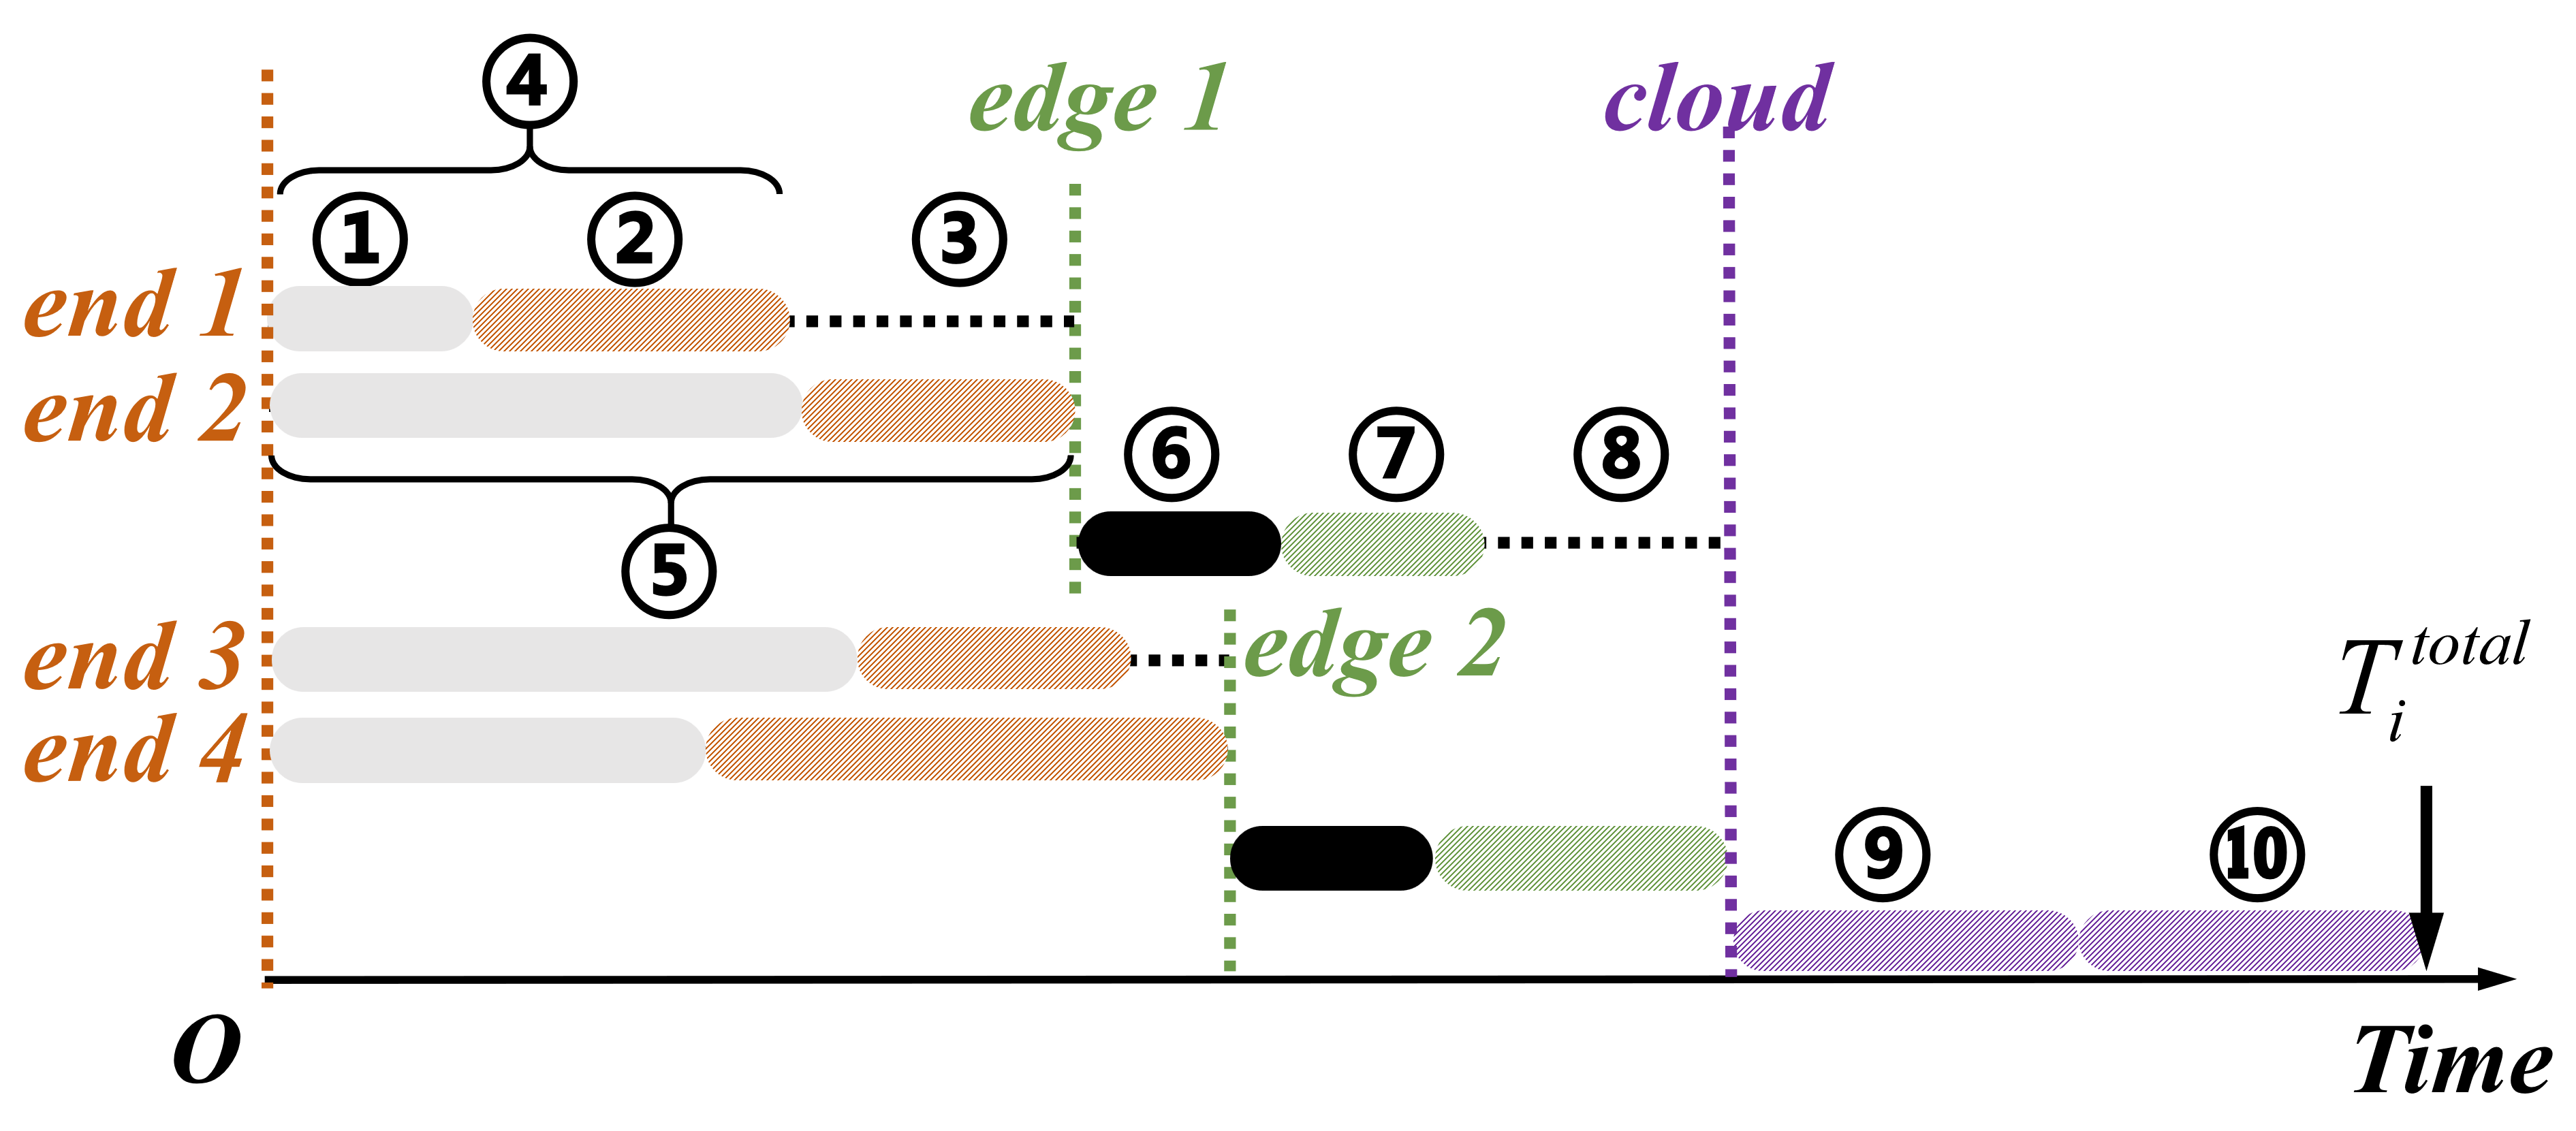
\includegraphics[width=\columnwidth]{time.png}
\caption{Path level Flow latency decomposition for an end device in cloud-edge-end hierarchical FL.}
\label{fig:time}
\end{figure}

\replaced[id=R1]{Fig.~\ref{fig:time} illustrates how the compact latency model in \equref{eq:latency_model} is instantiated in a representative complete end-edge-cloud Flow.}{Fig.~\ref{fig:time} illustrates the latency components of one communication round in hierarchical FL.}
\added[id=R1]{Marker \textcircled{1} denotes the local model training time of the end device, corresponding to \(T_i^{\mathrm{lupd}}(h_i,\mathcal{P}_i)\).}
\added[id=R1]{Marker \textcircled{2} denotes the communication time for uploading the local model, intermediate representation, or update to the associated edge server, corresponding to \(T_{i,j}^{\mathrm{comm},t}(h_i,\mathcal{P}_i)\).}
\added[id=R1]{Marker \textcircled{3} denotes the waiting time after the upload is completed and before the edge server starts aggregation, corresponding to \(W_{i,j}^{\mathrm{agg},t}\).}
\added[id=R1]{Marker \textcircled{4} denotes the arrival time at the edge server:}
\begin{equation}
x_{i,j}^{t}
=
T_i^{\mathrm{lupd}}(h_i,\mathcal{P}_i)
+
T_{i,j}^{\mathrm{comm},t}(h_i,\mathcal{P}_i).
\end{equation}
\added[id=R1]{Marker \textcircled{5} denotes the start time of local edge aggregation, which is determined by the latest arrival among the selected buffered aggregation set \(S_j^t\):}
\begin{equation}
X_j^{t}
=
\max_{i\in S_j^t}x_{i,j}^{t}.
\end{equation}
\added[id=R1]{Marker \textcircled{6} denotes the edge aggregation time, corresponding to \(T_j^{\mathrm{agg},t}\).}
\added[id=R1]{Marker \textcircled{7} denotes the communication time for uploading the edge aggregated model to the cloud server, corresponding to \(T_{j\rightarrow c}^{\mathrm{comm},t}\).}
\added[id=R1]{Marker \textcircled{8} denotes the waiting time after the edge server completes uploading and before the cloud server starts global aggregation, corresponding to \(W_{j,c}^{\mathrm{agg},t}\).}
\added[id=R1]{Marker \textcircled{9} denotes the cloud global aggregation and model return stage, including the cloud aggregation time \(T_c^{\mathrm{agg},t}\) and the cloud-to-edge download time \(T_{c\rightarrow j}^{\mathrm{comm},t}\).}
\added[id=R1]{Marker \textcircled{10} denotes the communication time for returning the updated global model from the edge server to the end device, corresponding to \(T_{j\rightarrow i}^{\mathrm{comm},t}\).}

\replaced[id=R1]{For the complete path across the end, edge, and cloud layers in \figref{fig:time}, the path level latency \(T_i(h_i,\mathcal{P}_i)\) can be expanded as}{For the complete path across the end, edge, and cloud layers in \figref{fig:time}, the total latency can be expanded as}
\begin{equation}
\begin{aligned}
\replaced[id=R1]{T_i(h_i,\mathcal{P}_i)}{T_i^{\mathrm{total}}}
=&\;
T_i^{\mathrm{lupd}}(h_i,\mathcal{P}_i)
+T_{i,j}^{\mathrm{comm},t}(h_i,\mathcal{P}_i)
+W_{i,j}^{\mathrm{agg},t}
+T_j^{\mathrm{agg},t}\\
&+T_{j\rightarrow c}^{\mathrm{comm},t}
+W_{j,c}^{\mathrm{agg},t}
+T_c^{\mathrm{agg},t}
+T_{c\rightarrow j}^{\mathrm{comm},t}
+T_{j\rightarrow i}^{\mathrm{comm},t}.
\end{aligned}
\label{eq:path_total_latency}
\end{equation}
\added[id=R1]{This expanded expression is a concrete instance of \equref{eq:latency_model}.} For modes that do not pass through the cloud or do not contain two level aggregation, the corresponding communication, waiting, and aggregation terms are set to zero.

DP budget refers specifically to the \(\epsilon\)-budget of differential privacy and is consumed only by interaction links where DP is enabled.
If a privacy sensitive link does not use DP, it is protected by HE instead.
\replaced[id=R1]
{HE does not consume the DP \(\epsilon\)-budget, but it still provides privacy protection and enters the latency model through ciphertext expansion and additional encryption and decryption processing overhead.}
{HE does not consume the DP \(\epsilon\)-budget, but it still provides privacy protection and enters the latency model through ciphertext expansion and encryption/decryption processing overhead.}

Let \(\epsilon_i^t\) be the remaining privacy budget of client \(i\) at the beginning of round \(t\).
The indicator
\begin{equation}
\mathbb{I}_{\mathrm{DP}}(b,h_i,\mathcal{P}_i)
=
\mathbb{I}\left(\sum_{u,v}\mathbf{I}_{b}^{h_i}(u,v)>0\right)
\mathbb{I}\left(\mathrm{DP}\in\mathcal{P}_i(b)\right)
\end{equation}
indicates that transmission type \(b\) occurs under mode \(h_i\) and is protected by DP.
By the basic sequential composition property of DP~\cite{dwork2014the}, the single round budget consumption is
\begin{equation}
    \epsilon_i^{\mathrm{used}}(h_i,\mathcal{P}_i)
    =
    \replaced[id=R1]{\sum_{b\in\mathcal{B}}
    N_b(h_i)\mathbb{I}_{\mathrm{DP}}(b,h_i,\mathcal{P}_i)\epsilon_b}
    {\sum_{\lambda\in\mathcal{E}_{\mathrm{flow}}^{h_i}}
    N_{\lambda}(h_i)\mathbb{I}_{\mathrm{DP}}(b_{\lambda},h_i,\mathcal{P}_i)\epsilon_{b_{\lambda}}}.
\label{eq:privacy_budget}
\end{equation}
\added[id=R1]{Here, \(N_b(h_i)\) denotes the number of DP-sensitive transmissions of type \(b\) within one complete Flow under mode \(h_i\). It is not an optimization variable; it is determined by the Flow topology of \(h_i\), including repetitions caused by the local Block loop \(L_B\) and the edge aggregation loop \(E_B\). For split-training interactions, \(N_{\mathrm{emb}}(h_i)\) and \(N_{\mathrm{grad}}(h_i)\) scale with the number of repeated Blocks, while \(N_{\mathrm{upd}}(h_i)\) is determined by the number of update upload and model return stages in the selected Flow.}
The remaining budget is updated by \(\epsilon_i^{t+1}=\epsilon_i^t-\epsilon_i^{\mathrm{used}}\), and candidates satisfying \(\epsilon_i^{\mathrm{used}}\le\epsilon_i^t\) are privacy feasible.

Finally, we derive how privacy mechanisms enter the convergence error proxy.
The derivation is included here because the proxy is used directly in the mode selection objective.
Consider a model consisting of an encoder \(f_{\phi}\) and a classifier or trainer \(g_{\theta}\).
For a local sample \(x\), the encoder output is
\begin{equation}
    z=f_{\phi}(x)\in\mathbb{R}^{d_z}.
\end{equation}
Feature level DP first clips the representation and then injects Gaussian noise:
\begin{equation}
    z^{\mathrm{clip}}
    =
    \frac{z}{\max(1,\|z\|_2/C)},
    \quad
    \tilde{z}=z^{\mathrm{clip}}+\nu,
    \quad
    \nu\sim\mathcal{N}(0,\sigma^2C^2I_{d_z}).
\label{eq:feature_dp_noise}
\end{equation}
For a linear prediction head \(o=W_{\mathrm{clf}}\tilde{z}+b\) and a softmax cross entropy loss \(\ell(\theta;\tilde{z})\), a second order Taylor expansion around the noise free point gives
\begin{equation}
\mathbb{E}_{\nu}[\ell(\theta;\tilde{z})]
\approx
\ell(\theta;z)
+\frac{\sigma^2C^2}{2}
\operatorname{Tr}\left(W_{\mathrm{clf}}^\top\nabla_o^2\ell W_{\mathrm{clf}}\right).
\label{eq:dp_loss_taylor}
\end{equation}
Since \(\nabla_o^2\ell=\operatorname{diag}(p)-pp^\top\) for \(p=\operatorname{softmax}(o)\), the DP induced loss inflation can be written as
\begin{equation}
    \Delta_{\mathrm{emb}}
    =
    \frac{\sigma^2C^2}{4}
    \sum_{j,k}p_jp_k
    \|W_{\mathrm{clf},j}-W_{\mathrm{clf},k}\|_2^2 .
\label{eq:delta_emb}
\end{equation}
This term shows that feature perturbation increases the expected local objective even when the injected noise has zero mean.

Feature level DP also affects the backward signal.
Let \(\Delta o=W_{\mathrm{clf}}\nu\) and \(\Sigma_o=\mathbb{E}[\Delta o\Delta o^\top]=\sigma^2C^2W_{\mathrm{clf}}W_{\mathrm{clf}}^\top\).
Expanding the perturbed softmax probability \(\tilde{p}\) to second order yields
\begin{equation}
\mathbb{E}_{\nu}[\tilde{p}_r]
\approx
p_r+\frac{1}{2}\operatorname{Tr}(H^{(r)}\Sigma_o),
\end{equation}
where \(H^{(r)}\) is the Hessian of the \(r\)-th softmax output with respect to logits.
Define the bias vector
\begin{equation}
    [\mathbf{b}_{\mathrm{bias}}]_r
    =
    \frac{1}{2}\operatorname{Tr}(H^{(r)}\Sigma_o).
\end{equation}
Then the expected gradient with respect to the transmitted representation satisfies
\begin{equation}
\mathbb{E}_{\nu}\left[\frac{\partial\ell}{\partial \tilde{z}}\right]
\approx
W_{\mathrm{clf}}^\top(p-y)
+W_{\mathrm{clf}}^\top\mathbf{b}_{\mathrm{bias}}.
\label{eq:feature_dp_bias}
\end{equation}
Thus, feature level DP introduces not only variance but also a systematic gradient bias with magnitude
\begin{equation}
    \zeta=\|W_{\mathrm{clf}}^\top\mathbf{b}_{\mathrm{bias}}\|_2 .
\label{eq:zeta_bias}
\end{equation}

For update level DP, the client update vector
\(u_i^t=\operatorname{vec}(\theta_i^t-w_s^t)\) is clipped and perturbed:
\begin{equation}
    u_i^{t,\mathrm{clip}}
    =
    \frac{u_i^t}{\max(1,\|u_i^t\|_2/C_u)},
    \quad
    \tilde{u}_i^t=u_i^{t,\mathrm{clip}}+\xi_i^t,
    \quad
    \xi_i^t\sim\mathcal{N}(0,\sigma_u^2C_u^2I_d).
\label{eq:update_dp_noise}
\end{equation}
After aggregation over the participating set \(\mathcal{A}_s^{(t)}\), the update noise contributes the variance term
\begin{equation}
    \mathbb{E}\|\tilde{u}_s^t-\bar{u}_s^t\|_2^2
    \propto
    \frac{\sigma_u^2C_u^2d}{|\mathcal{A}_s^{(t)}|^2}.
\label{eq:update_dp_variance}
\end{equation}

We assume that the global objective \(F(w)\) is \(G\)-smooth and satisfies the \(\mu\)-PL condition
\(\|\nabla F(w)\|_2^2\ge 2\mu(F(w)-F(w^*))\).
Combining the feature bias, loss inflation, local stochastic variance, and update DP variance gives a one step recursion
\begin{equation}
\mathbb{E}[F(w^{t+1})-F(w^*)]
\le
(1-\rho_{\mathrm{PL}})\mathbb{E}[F(w^t)-F(w^*)]
+\mathcal{R}(h_i,\mathcal{P}_i).
\label{eq:pl_recursion}
\end{equation}
Taking the steady state of this recursion gives
\(\lim_{t\to\infty}\mathbb{E}[F(w^t)-F(w^*)]\approx \mathcal{R}(h_i,\mathcal{P}_i)/\rho_{\mathrm{PL}}\).
Let \(\mathbb{I}_{\mathrm{emb}}^{i,t}\) and \(\mathbb{I}_{\mathrm{upd}}^{i,t}\) indicate whether client \(i\) enables DP for intermediate features and model updates in round \(t\).
The local convergence error proxy is then defined as
\begin{equation}
\begin{aligned}
    \widehat{\Omega}(h_i,\mathcal{P}_i)
    &\approx \lim_{t \to \infty}\mathbb{E}[F(w^t)-F(w^*)]
    = \frac{\mathcal{R}(h_i,\mathcal{P}_i)}{\rho_{\mathrm{PL}}} \\
    &= \frac{3}{2\mu}\left(\mathbb{I}_{\mathrm{emb}}^{i,t}\|W_{\mathrm{clf}}^\top \mathbf{b}_{\mathrm{bias}}\|_2^2
    + \mathbb{I}_{\mathrm{emb}}^{i,t}G \Delta_{\mathrm{emb}}\right) \\
    &\quad + \frac{G\eta_{\mathrm{lr}} L_B}{\mu}\left(\sigma_{\mathrm{local}}^2
    + \mathbb{I}_{\mathrm{upd}}^{i,t}\frac{\sigma_u^2C_u^2d}{\eta_{\mathrm{lr}}^2L_B^2|\mathcal{A}_s^{(t)}|^2}\right).
\end{aligned}
\label{eq:local_omega}
\end{equation}
Here, \(\rho_{\mathrm{PL}}\) is the contraction factor associated with the PL based convergence proxy, and \(\eta_{\mathrm{lr}}\) is the learning rate.
This proxy measures the theoretical effect of privacy perturbation and local training instability.
It is not a direct prediction of real test accuracy.

\subsection{Global Multi Objective Collaborative Optimization}
\label{sec:global_optimization}
The previous subsection defines the resource feasibility, path level latency, privacy budget, and local convergence error proxy for one device.
Cloud-edge-end FL ultimately trains a system level global model.
If each device independently selects the fastest or locally lowest error mode, cross edge information fusion may be insufficient, especially under non-IID data.
Let \(\mathbf{h}_{\mathcal{N}}=[h_1,\dots,h_N]\) and \(\boldsymbol{\mathcal{P}}_{\mathcal{N}}=[\mathcal{P}_1,\dots,\mathcal{P}_N]\) denote the global mode and privacy policy vectors.

Path level latency \(T_i\) describes one device's end to end Flow, whereas system round latency \(T_{\mathrm{sys}}\) describes when one federated communication round completes.
Under synchronous aggregation or a determined buffered set,
\begin{equation}
T_{\mathrm{sys}}(\mathbf{h}_{\mathcal{N}},\boldsymbol{\mathcal{P}}_{\mathcal{N}})
= \max_{i\in\mathcal{A}^{(t)}} T_i(h_i,\mathcal{P}_i),
\label{eq:global_latency}
\end{equation}
where \(\mathcal{A}^{(t)}\) is the set of devices that reach the final aggregation node in round \(t\).

Let the set of cloud involved modes be
\begin{equation}
\mathcal{H}_C=\{\mathrm{LIC},\mathrm{LIIC},\mathrm{LIEIIC},\mathrm{LIEIIIC},\mathrm{LIIEIIIC}\}.
\end{equation}
The cloud fusion ratio is
\begin{equation}
r_C(\mathbf{h}_{\mathcal{N}})
=
\frac{\sum_{i=1}^{N} n_i\mathbb{I}(h_i\in\mathcal{H}_{C})}{N_{\mathrm{total}}},
\quad
N_{\mathrm{total}}=\sum_{i=1}^{N}n_i.
\end{equation}
It measures the sample proportion participating in cloud level cross edge fusion.
To penalize insufficient cloud fusion, we define
\begin{equation}
\Psi_C(\mathbf{h}_{\mathcal{N}})
:=
\frac{\xi}{r_C(\mathbf{h}_{\mathcal{N}})+\varepsilon},
\label{eq:cloud_penalty}
\end{equation}
where \(\xi\) controls penalty strength and \(\varepsilon\) avoids division by zero.
The system level global convergence error proxy is
\begin{equation}
\widehat{\Omega}_{\mathrm{sys}}(\mathbf{h}_{\mathcal{N}},\boldsymbol{\mathcal{P}}_{\mathcal{N}})
=
\sum_{i=1}^{N}
\frac{n_i}{N_{\mathrm{total}}}
\widehat{\Omega}(h_i,\mathcal{P}_i)
+\Psi_C(\mathbf{h}_{\mathcal{N}}).
\label{eq:global_omega}
\end{equation}
When many devices remain in edge only modes such as LIE or LIIE, \(r_C\) decreases and the cross edge fusion penalty increases.
This term models the theoretical risk of insufficient global information exchange; it does not imply that cloud paths always have better local accuracy.

We use ideal point approximation to scalarize latency and global convergence error proxy:
\begin{equation}
\begin{aligned}
\min_{\mathbf{h}_{\mathcal{N}},\boldsymbol{\mathcal{P}}_{\mathcal{N}}} \quad
& \Bigg[
\omega_T\left(\frac{T_{\mathrm{sys}}-T_{\min}}{T_{\max}-T_{\min}}\right)^2
+
\omega_{\Omega}\left(\frac{\widehat{\Omega}_{\mathrm{sys}}-\widehat{\Omega}_{\min}}{\widehat{\Omega}_{\max}-\widehat{\Omega}_{\min}}\right)^2
\Bigg]^{1/2}\\
\mathrm{s.t.}\quad
& h_i\in\mathcal{H}_i,\quad \mathcal{P}_i\in\Pi(h_i),\quad \forall i\in\mathcal{N},\\
& C_i^{\mathrm{comp}}(h_i,n_i,m_i)\le Q_{c,i},\quad C_i^{\mathrm{mem}}(h_i)\le Q_{e,i},\quad \forall i\in\mathcal{N},\\
& \epsilon_i^{\mathrm{used}}(h_i,\mathcal{P}_i)\le \epsilon_i^t,\quad \forall i\in\mathcal{N}.
\end{aligned}
\label{eq:selection}
\end{equation}
Real test accuracy is not included in the objective function and is only used in experiments to evaluate the empirical effect of the proxy objective.

\begin{figure}[t]
\centering
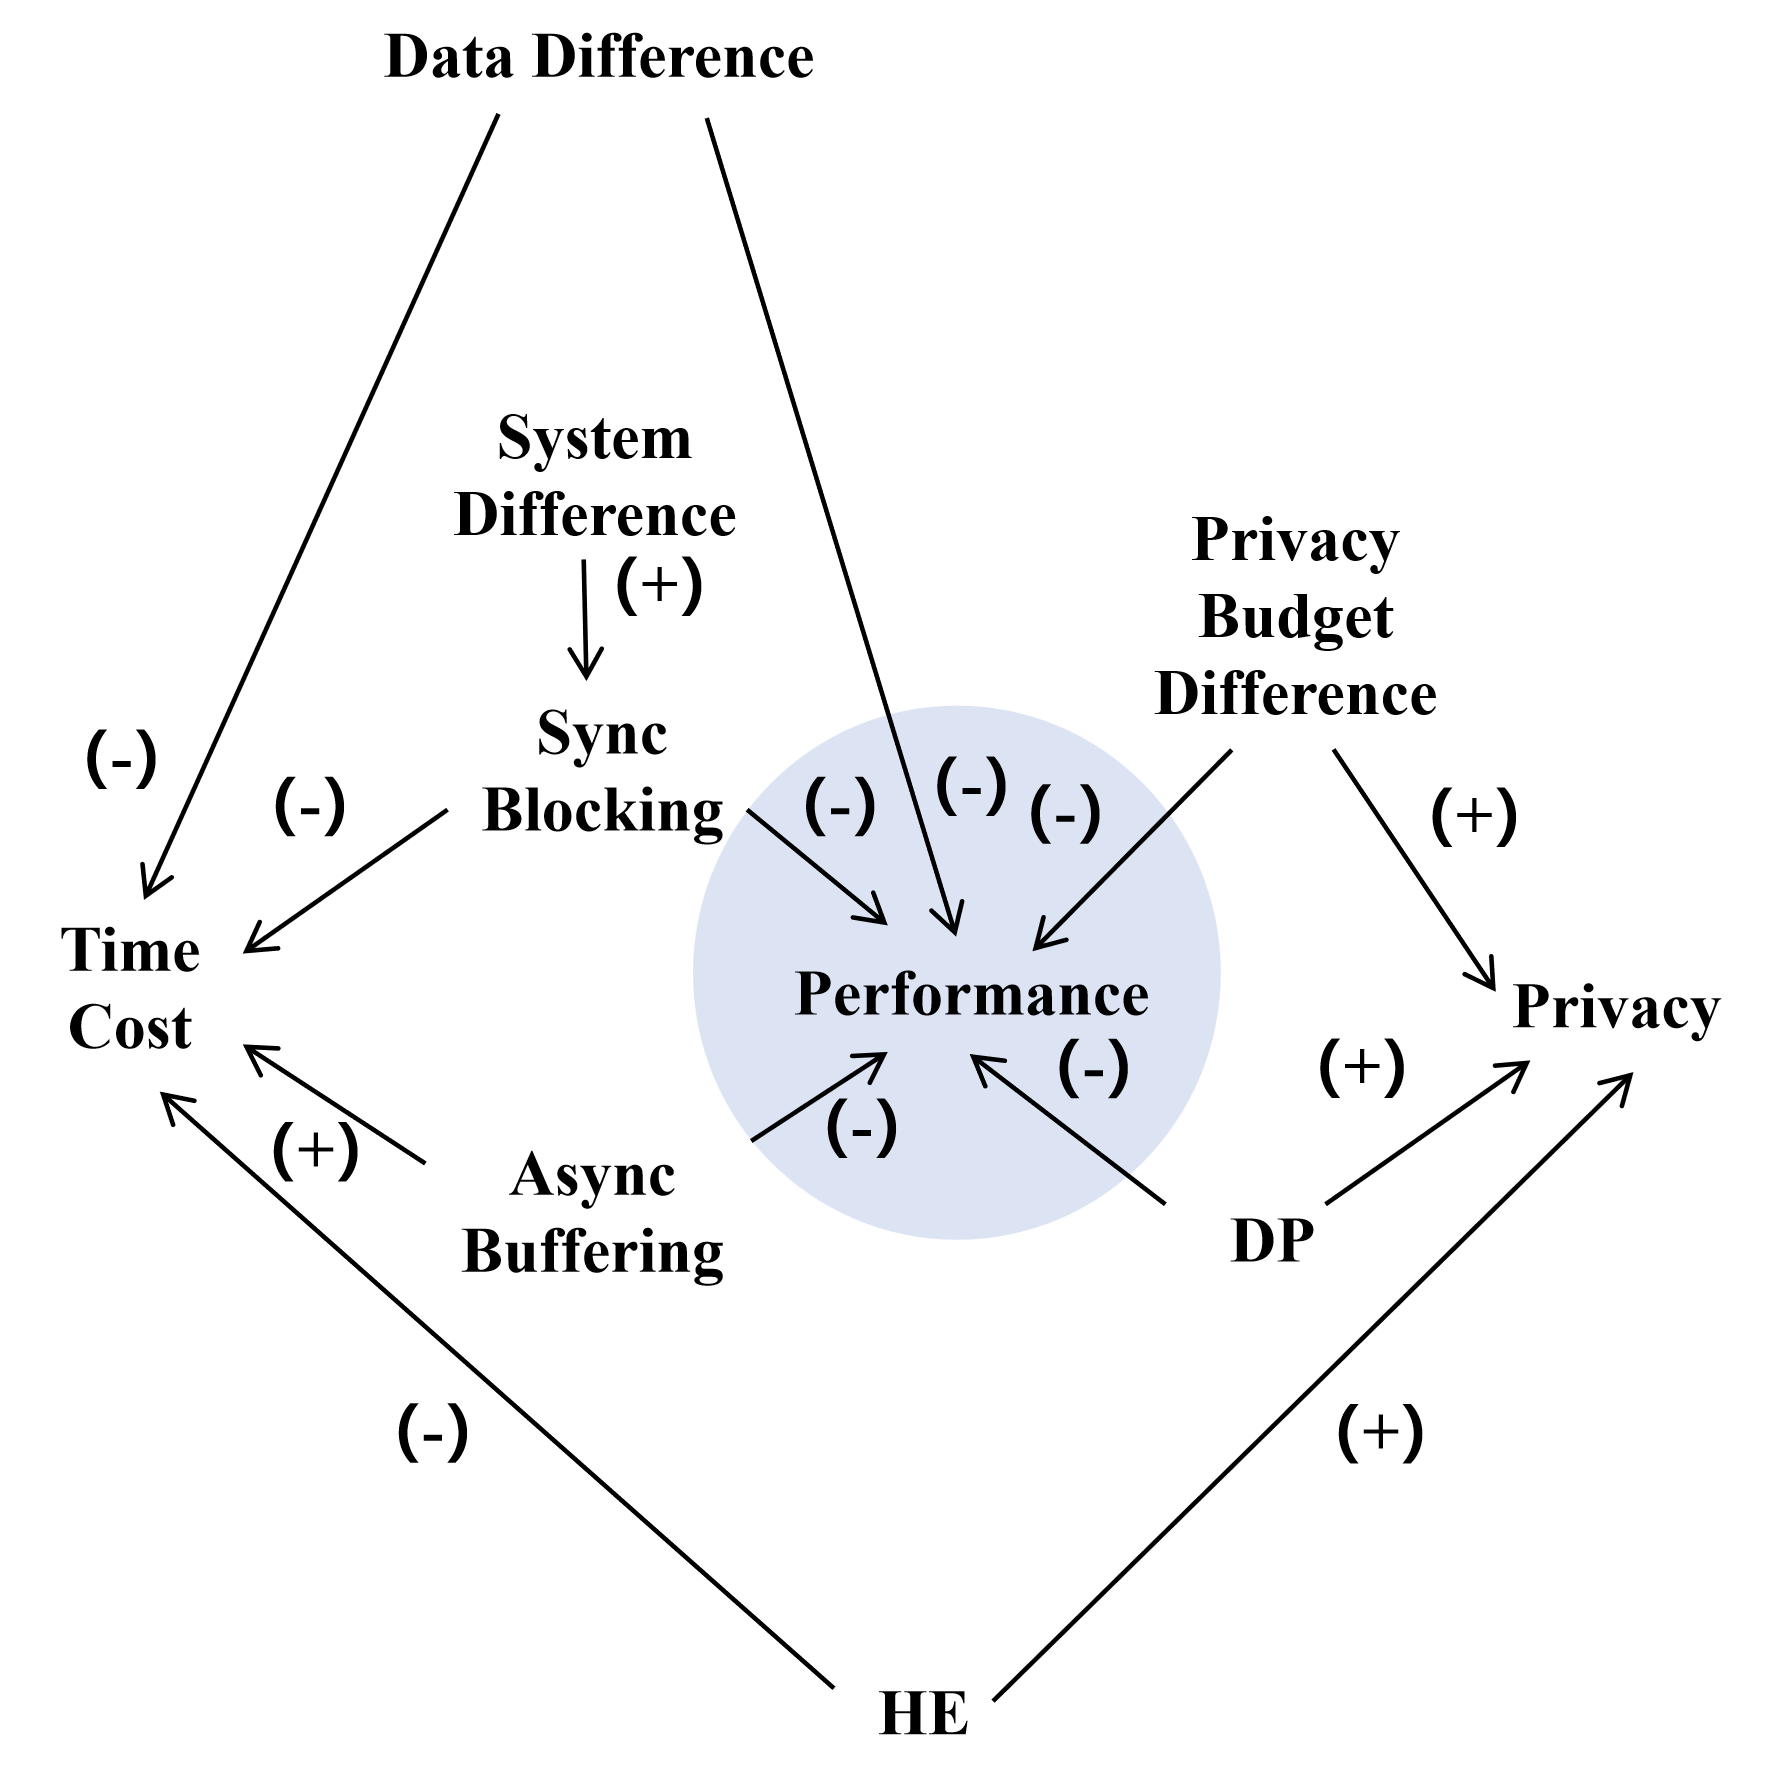
\includegraphics[width=\columnwidth]{balance.png}
\caption{Interaction among privacy protection, training efficiency, and the convergence error proxy.}
\label{fig:balance}
\end{figure}

\section{Algorithm}
\label{sec:algorithm}
\begin{table*}[t]
\caption{Main Notation}
\label{tab:notations}
\centering
\begin{tabular}{p{0.25\textwidth}p{0.69\textwidth}}
\hline\hline
\textbf{Symbol} & \textbf{Meaning} \\
\hline
\(\mathcal{N}, N\) & End device set and number of end devices \\
\(\mathcal{H}, \mathcal{H}_i\) & Global candidate hierarchical mode set and resource feasible mode set of client \(i\) \\
\(\Pi(h_i), \mathcal{P}_i\) & Candidate privacy policy set under mode \(h_i\), and the policy selected by client \(i\) \\
\(s_i=(h_i,\mathcal{P}_i),\mathcal{S}_i\) & One decision pair of client \(i\), and the feasible candidate set \\
\(L_B,E_B\) & Number of local Block loops and number of edge aggregation loops before cloud aggregation \\
\(Q_{c,i}, Q_{e,i}\) & Local computation budget and memory upper bound of client \(i\) \\
\(\epsilon_i^t\) & Remaining DP budget of client \(i\) at the beginning of round \(t\) \\
\(C_i^{\mathrm{comp}}, C_i^{\mathrm{mem}}\) & Computation and memory costs of client \(i\) under a selected mode \\
\(\epsilon_i^{\mathrm{used}}\) & DP budget consumed by one complete Flow \\
\(T_i, T_{\mathrm{sys}}\) & Path level Flow latency of client \(i\), and system level round latency \\
\added[id=R1]{\(C_i^{\mathrm{sw},t}, S_P\) & Mode switching overhead in round \(t\), and strategy update period for limiting reconfiguration frequency \\}
\(S_j^t,\lvert S_j^t\rvert\) & Set of client updates selected into edge aggregator \(j\)'s buffered aggregation in round \(t\), and the number of selected updates \\
\(S_{\mathrm{agg}}^t\) & Equivalent data size of one selected client update in aggregation computation \\
\(\widehat{\Omega}_i, \widehat{\Omega}_{\mathrm{sys}}\) & Local convergence error proxy and global convergence error proxy \\
\(\Psi_C, r_C\) & Cloud fusion insufficiency penalty and cloud fusion ratio \\
\(\rho_{\mathrm{buf}},\rho_{\mathrm{PL}}\) & Buffered aggregation participation threshold and PL based convergence contraction factor \\
\(\eta_{\mathrm{lr}},\nu\) & Learning rate and Gaussian noise added to intermediate features by feature level DP \\
\(\Delta_{\mathrm{emb}},W_{\mathrm{clf}}\) & Feature level DP loss inflation term and local classifier weight matrix \\
\hline\hline
\end{tabular}
\end{table*}

The dynamic hierarchical mode selection process contains two stages.
First, each device constructs a candidate decision set \(\mathcal{S}_i\) by filtering resource feasible hierarchical modes and enumerating optional privacy mechanism assignments for intermediate features and model updates.
Second, the system selects a global decision combination from \(\{\mathcal{S}_i\}_{i\in\mathcal{N}}\), computes \(T_{\mathrm{sys}}\), \(\widehat{\Omega}_{\mathrm{sys}}\), and \(r_C\), and chooses the combination closest to the ideal reference point in \equref{eq:selection}.
\added[id=R1]{When switching overhead is considered, candidate evaluation also conditions on the previous decision \((h_i^{t-1},\mathcal{P}_i^{t-1})\), and \(T_i\) includes \(C_i^{\mathrm{sw},t}\) in \equref{eq:latency_model}. To avoid excessive reconfiguration, the selection step can be triggered every \(S_P\) rounds. If \(t\) is not a strategy update point, the previous mode and privacy assignment are reused and only the remaining resource and privacy states are updated.}
The experiments use a greedy rebalancing solver: each device first selects the local candidate with the smallest normalized distance, and then devices are replaced with cloud involved candidates according to \(r_C\) and \(\widehat{\Omega}_{\mathrm{sys}}\) until the global objective no longer decreases or a maximum number of updates is reached.
If each device has at most \(K_{\mathrm{cand}}\le|\mathcal{H}||\Pi|\) candidates, candidate construction has complexity \(O(NK_{\mathrm{cand}})\), and sorting plus rebalancing has complexity \(O(NK_{\mathrm{cand}}\log K_{\mathrm{cand}})\).

\begin{algorithm}[t]
\caption{Privacy Aware Dynamic Hierarchical Mode Selection (\method)}
\label{alg:selection}
\begin{algorithmic}[1]
\REQUIRE End device set \(\mathcal{N}\), candidate modes \(\mathcal{H}\), privacy mechanism assignments \(\Pi\), resource budgets \(Q_{c,i},Q_{e,i}\), remaining DP budget \(\epsilon_i^t\), weights \(\omega_T,\omega_\Omega\)\added[id=R1]{, previous decisions \(\{(h_i^{t-1},\mathcal{P}_i^{t-1})\}_{i\in\mathcal{N}}\), strategy update period \(S_P\)}
\ENSURE Global collaborative decisions \(\{(h_i^\star,\mathcal{P}_i^\star)\}_{i\in\mathcal{N}}\)
\added[id=R1]{\IF{\(t\) is not a strategy update point}
    \STATE Reuse \(\{(h_i^{t-1},\mathcal{P}_i^{t-1})\}_{i\in\mathcal{N}}\) and update only runtime states.
    \STATE \RETURN \(\{(h_i^{t-1},\mathcal{P}_i^{t-1})\}_{i\in\mathcal{N}}\).
\ENDIF}
\FOR{each device \(i\in\mathcal{N}\)}
    \STATE Build \(\mathcal{H}_i\) using computation and memory constraints.
    \STATE Initialize \(\mathcal{S}_i\leftarrow\emptyset\).
    \FOR{each feasible mode \(h_i\in\mathcal{H}_i\)}
        \FOR{each privacy mechanism assignment \(\mathcal{P}_i\in\Pi(h_i)\)}
            \STATE Compute \(\epsilon_i^{\mathrm{used}}(h_i,\mathcal{P}_i)\).
            \IF{\(\epsilon_i^{\mathrm{used}}\le\epsilon_i^t\)}
                \STATE Estimate \(T_i\) and \(\widehat{\Omega}_i\)\added[id=R1]{, including \(C_i^{\mathrm{sw},t}\) if switching overhead is enabled}.
                \STATE Add \((h_i,\mathcal{P}_i,T_i,\widehat{\Omega}_i)\) to \(\mathcal{S}_i\).
            \ENDIF
        \ENDFOR
    \ENDFOR
    \IF{\(\mathcal{S}_i=\emptyset\)}
        \STATE Mark client \(i\) as skipped in the current round.
    \ENDIF
\ENDFOR
\STATE Collect \(\mathcal{S}\leftarrow\{\mathcal{S}_i\}_{i\in\mathcal{N},\mathcal{S}_i\neq\emptyset}\).
\STATE Obtain \(T_{\min},T_{\max},\widehat{\Omega}_{\min},\widehat{\Omega}_{\max}\) from \(\mathcal{S}\).
\STATE Solve \equref{eq:selection} using greedy rebalancing.
\STATE \RETURN \(\{(h_i^\star,\mathcal{P}_i^\star)\}_{i\in\mathcal{N}}\).
\end{algorithmic}
\end{algorithm}

\section{Experiments}
\label{sec:experiment}
\subsection{Experimental Setup}
\label{sec:exp_setup}
\textbf{Simulation environment and parameters.}
We build a Python 3.10 cloud-edge-end FL simulation system with end devices, edge nodes, and a cloud node.
The default simulation parameters are shown in \tabref{tab:sim_params}.
Resource constraints apply only to the submodel actually undertaken by the end device.
End devices do not need to satisfy the hardware requirement of training the full model, but they must at least support the encoder side Block.
Edge servers are assumed to have higher aggregation and collaborative computation capacity than their attached end devices, and the cloud is treated as non bottleneck.

\begin{table}[t]
\centering
\caption{Default Simulation Parameters}
\label{tab:sim_params}
\begin{tabular}{lc}
\hline
\textbf{Parameter} & \textbf{Value or Description} \\
\hline
End / edge nodes & \(N=100\) / \(E=10\) \\
Training rounds & \(T=50\) \\
Device type ratio & weak 40\%, medium 35\%, strong 25\% \\
Edge / cloud computation rate & 12.0 / 1000.0 \\
Local Block loops & \(L=5\) \\
Edge aggregation loops & 3 \\
Initial DP budget & \(\epsilon_0=4.0\) \\
Single DP event budget & \(\epsilon_{\mathrm{emb}}=0.03\), \(\epsilon_{\mathrm{upd}}=0.05\) \\
Base transmission size & \(S_{\mathrm{emb}}=1.6\) MB, \(S_{\mathrm{upd}}=4.0\) MB \\
HE expansion factor & \(\alpha_{\mathrm{HE}}=6.0\) \\
Network jitter coefficient & 0.25 \\
Edge pre aggregation reduction & 0.55 \\
\hline
\end{tabular}
\end{table}

The budgets \(\epsilon_{\mathrm{emb}}\) and \(\epsilon_{\mathrm{upd}}\) are per event DP costs for different transmission objects.
The end device only needs the total DP cost of all DP protected transmissions in one Flow to be no greater than its current remaining budget.
The base transmission sizes are not fixed communication volumes; the actual communication volume changes with the number of transmission links in the selected Flow and the privacy expansion factor.
The HE expansion factor \(\alpha_{\mathrm{HE}}=6.0\) simulates high cost encrypted transmission rather than a fixed constant for a specific HE implementation.
HE does not consume DP budget, but it increases communication and latency.
The network jitter coefficient introduces round level link rate fluctuations around the base rate.
The cloud fusion ratio \(r_C\) is an observed metric induced by selected modes rather than a predetermined target.

\textbf{Real training experiments.}
The original real training experiment uses Fashion-MNIST image classification with LeNet-5.
We sample 12000 training images and 2000 test images to control the cost of multiple policy comparison while keeping a real non-IID client training process.
There are 10 end devices, 2 edge nodes, 50 FL rounds, 1 local epoch, learning rate 0.15, and \(10^{-4}\) \(L_2\) weight decay.
The initial DP budget is \(\epsilon_0=10.0\), the single DP event cost is 0.01, the clipping threshold is 20.0, and the noise multiplier is 0.001.

\textbf{CIFAR-10 extension.}
To prepare the IoTJ English submission with stronger vision model evidence, we also summarize the newer CIFAR-10/ResNet-18 experiments.
These experiments use 200 rounds under cloud-edge-end simulation and compare \method{} with Fixed-HFL, Fixed-DP, No-Protection, Individual-Optimal, and Random.
They cover extreme edge label skew, IID, client non-IID, edge label skew, resource heterogeneity, strategy update period, aggregation fraction, and three random seeds.
HE related results are interpreted as a simulated overhead model, not as an end to end real encrypted training implementation.

\textbf{Baselines.}
\method{} uses the ideal point approximation in \equref{eq:selection}.
The original simulation compares Latency-Opt, Utility-Opt, Fixed-DP, Fixed-HE, No-Protection, and Random.
Latency-Opt chooses the feasible combination with minimum estimated latency.
Utility-Opt chooses the feasible combination with minimum local convergence error proxy.
Fixed-DP uniformly applies DP to related transmissions.
Fixed-HE forces model updates to use HE transmission.
Random randomly selects feasible hierarchical modes and privacy mechanisms.
The real training experiment reports Fixed-DP, Privacy-Only, No-Protection, and Random.
The CIFAR-10 extension uses Fixed-HFL, Fixed-DP, No-Protection, Individual-Optimal, and Random.

\textbf{Metrics.}
We evaluate latency, local convergence error proxy, active ratio, communication cost, DP budget consumption, cloud fusion ratio, global convergence error proxy, and test accuracy.
The logical time reported in real training tables is accumulated from candidate Flow computation, communication, waiting, and aggregation costs.
It is not wall clock runtime.

\subsection{System Level Simulation Results}
\label{sec:simulation_results}
\figref{fig:policy_comparison} shows the system level metric comparison under the default simulation configuration.
\method{} obtains a cloud fusion ratio of 0.456 and a global convergence error proxy of 0.132, lower than the latency only policy.
This indicates that after introducing the system level convergence error proxy, mode selection considers both end side latency and the risk of insufficient cross edge fusion, rather than simply selecting the fastest path.

\begin{figure}[t]
\centering
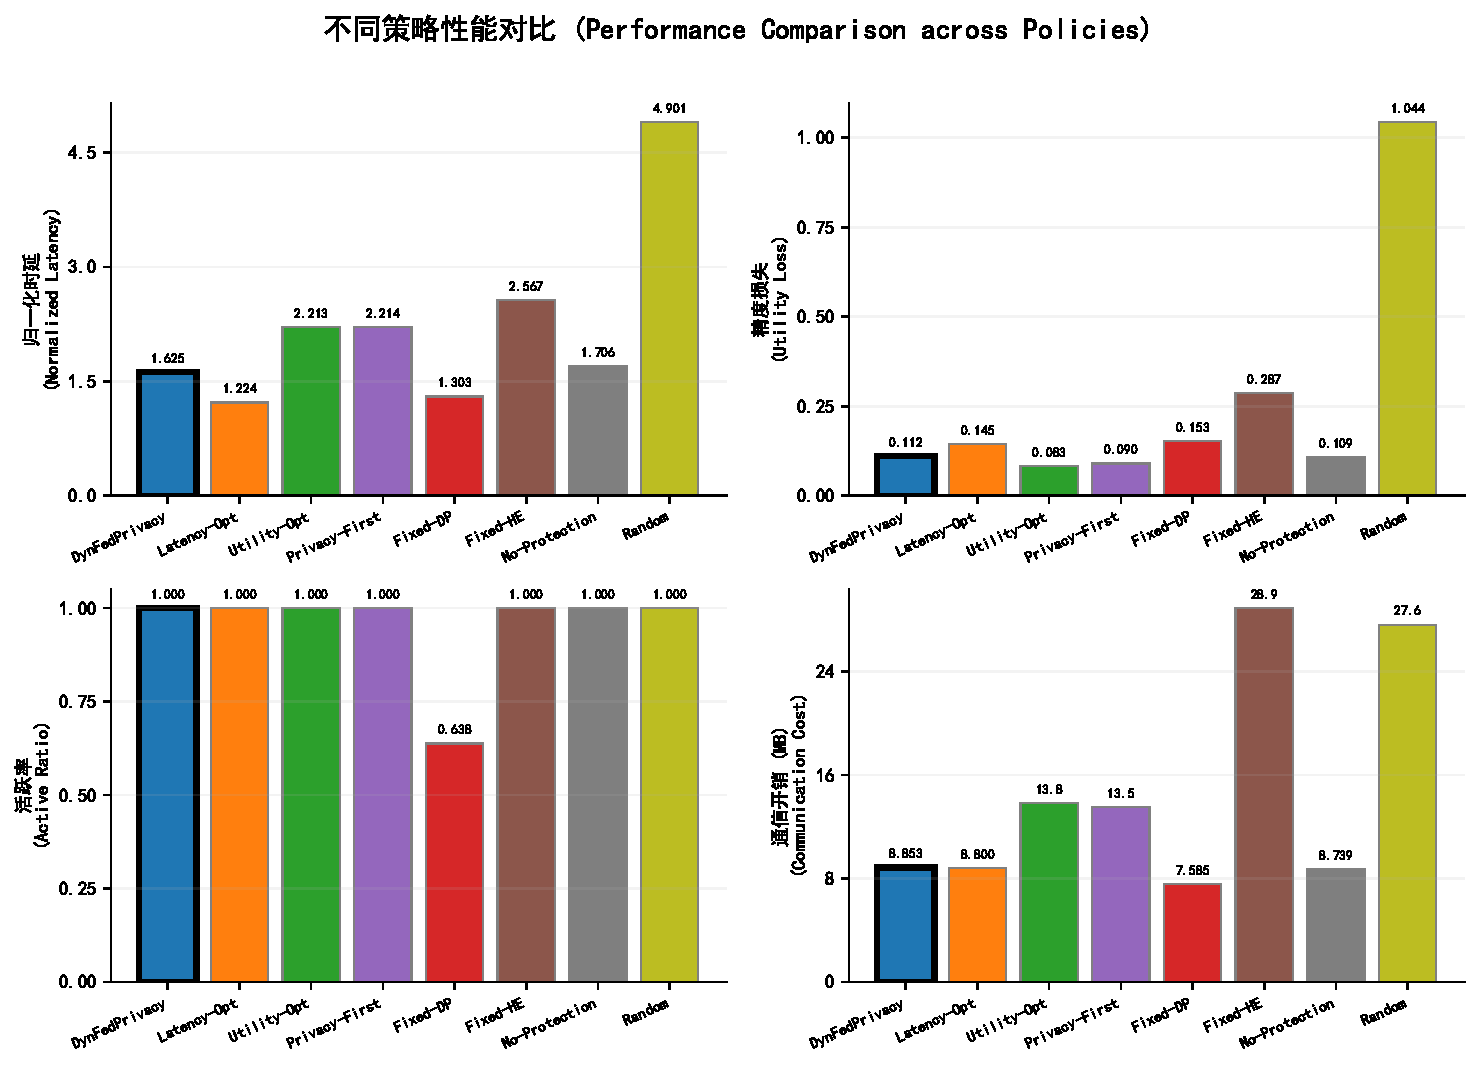
\includegraphics[width=\columnwidth]{fig1_policy_comparison.pdf}
\caption{System level metric comparison between \method{} and baseline policies.}
\label{fig:policy_comparison}
\end{figure}

\subsection{Fashion-MNIST Real Training Results}
\label{sec:fmnist_results}
\tabref{tab:real_comparison} reports 50 round LeNet-5 real FedAvg training on Fashion-MNIST.
\method{} reaches 63.25\% final accuracy and 72.80\% best accuracy, with logical time 355.20, communication 3398.23, and cumulative DP budget consumption 23.51.
The feasible active ratio remains 1.0 over all 50 rounds.
Compared with Fixed-DP, \method{} improves final accuracy by 2.25 percentage points and reduces logical time by 56.7\%.
The higher latency of Fixed-DP is not because DP itself is slower than HE, but because the fixed DP policy changes the feasible candidate set and causes more frequent selection of high cost paths with multiple level aggregation and waiting.
Privacy-Only, No-Protection, and Random obtain higher accuracy in this setting.
Therefore, the 50 round result should be interpreted cautiously: under the current weights, \method{} does not dominate all baselines in real test accuracy, but it provides better cost control than unconstrained random exploration and avoids the high cost of Fixed-DP.

\begin{table*}[t]
\centering
\caption{Performance Comparison on Fashion-MNIST with 50 Round LeNet-5 Real Training}
\label{tab:real_comparison}
\begin{tabular}{lccccc}
\hline
\textbf{Policy} & \textbf{Final Acc.} & \textbf{Best Acc.} & \textbf{Logical Time} & \textbf{Comm.} & \textbf{DP Budget} \\
\hline
\method{} & 0.632 & 0.728 & 355.198 & 3398.232 & 23.510 \\
Fixed-DP & 0.610 & 0.746 & 819.593 & 2861.712 & 24.220 \\
Privacy-Only & 0.779 & 0.779 & 144.329 & 3060.000 & 10.000 \\
No-Protection & 0.744 & 0.762 & 310.413 & 3222.400 & 0.000 \\
Random & 0.777 & 0.777 & 704.878 & 4181.184 & 22.320 \\
\hline
\end{tabular}
\end{table*}

\tabref{tab:real_extension} reports an additional real training experiment with 100 rounds and 3 local epochs.
\method{} achieves 70.40\% final accuracy and 80.10\% best accuracy, both higher than Privacy-Only.
Random reaches 80.05\% final accuracy and 82.05\% best accuracy, but its logical time and communication are the highest.
This confirms that random exploration can improve model utility in a longer training regime, but the absence of an objective constraint significantly increases system cost.

\begin{table}[t]
\centering
\caption{Supplementary Fashion-MNIST + LeNet-5 Experiment With 100 Rounds and 3 Local Epochs}
\label{tab:real_extension}
\begin{tabular}{lccccc}
\hline
\textbf{Policy} & \textbf{Final} & \textbf{Best} & \textbf{Time} & \textbf{Comm.} & \textbf{DP} \\
\hline
\method{} & 0.704 & 0.801 & 973.366 & 6793.608 & 46.500 \\
Privacy-Only & 0.669 & 0.726 & 627.220 & 6120.000 & 20.000 \\
Random & 0.800 & 0.821 & 1502.783 & 8203.656 & 44.090 \\
\hline
\end{tabular}
\end{table}

\begin{figure}[t]
\centering
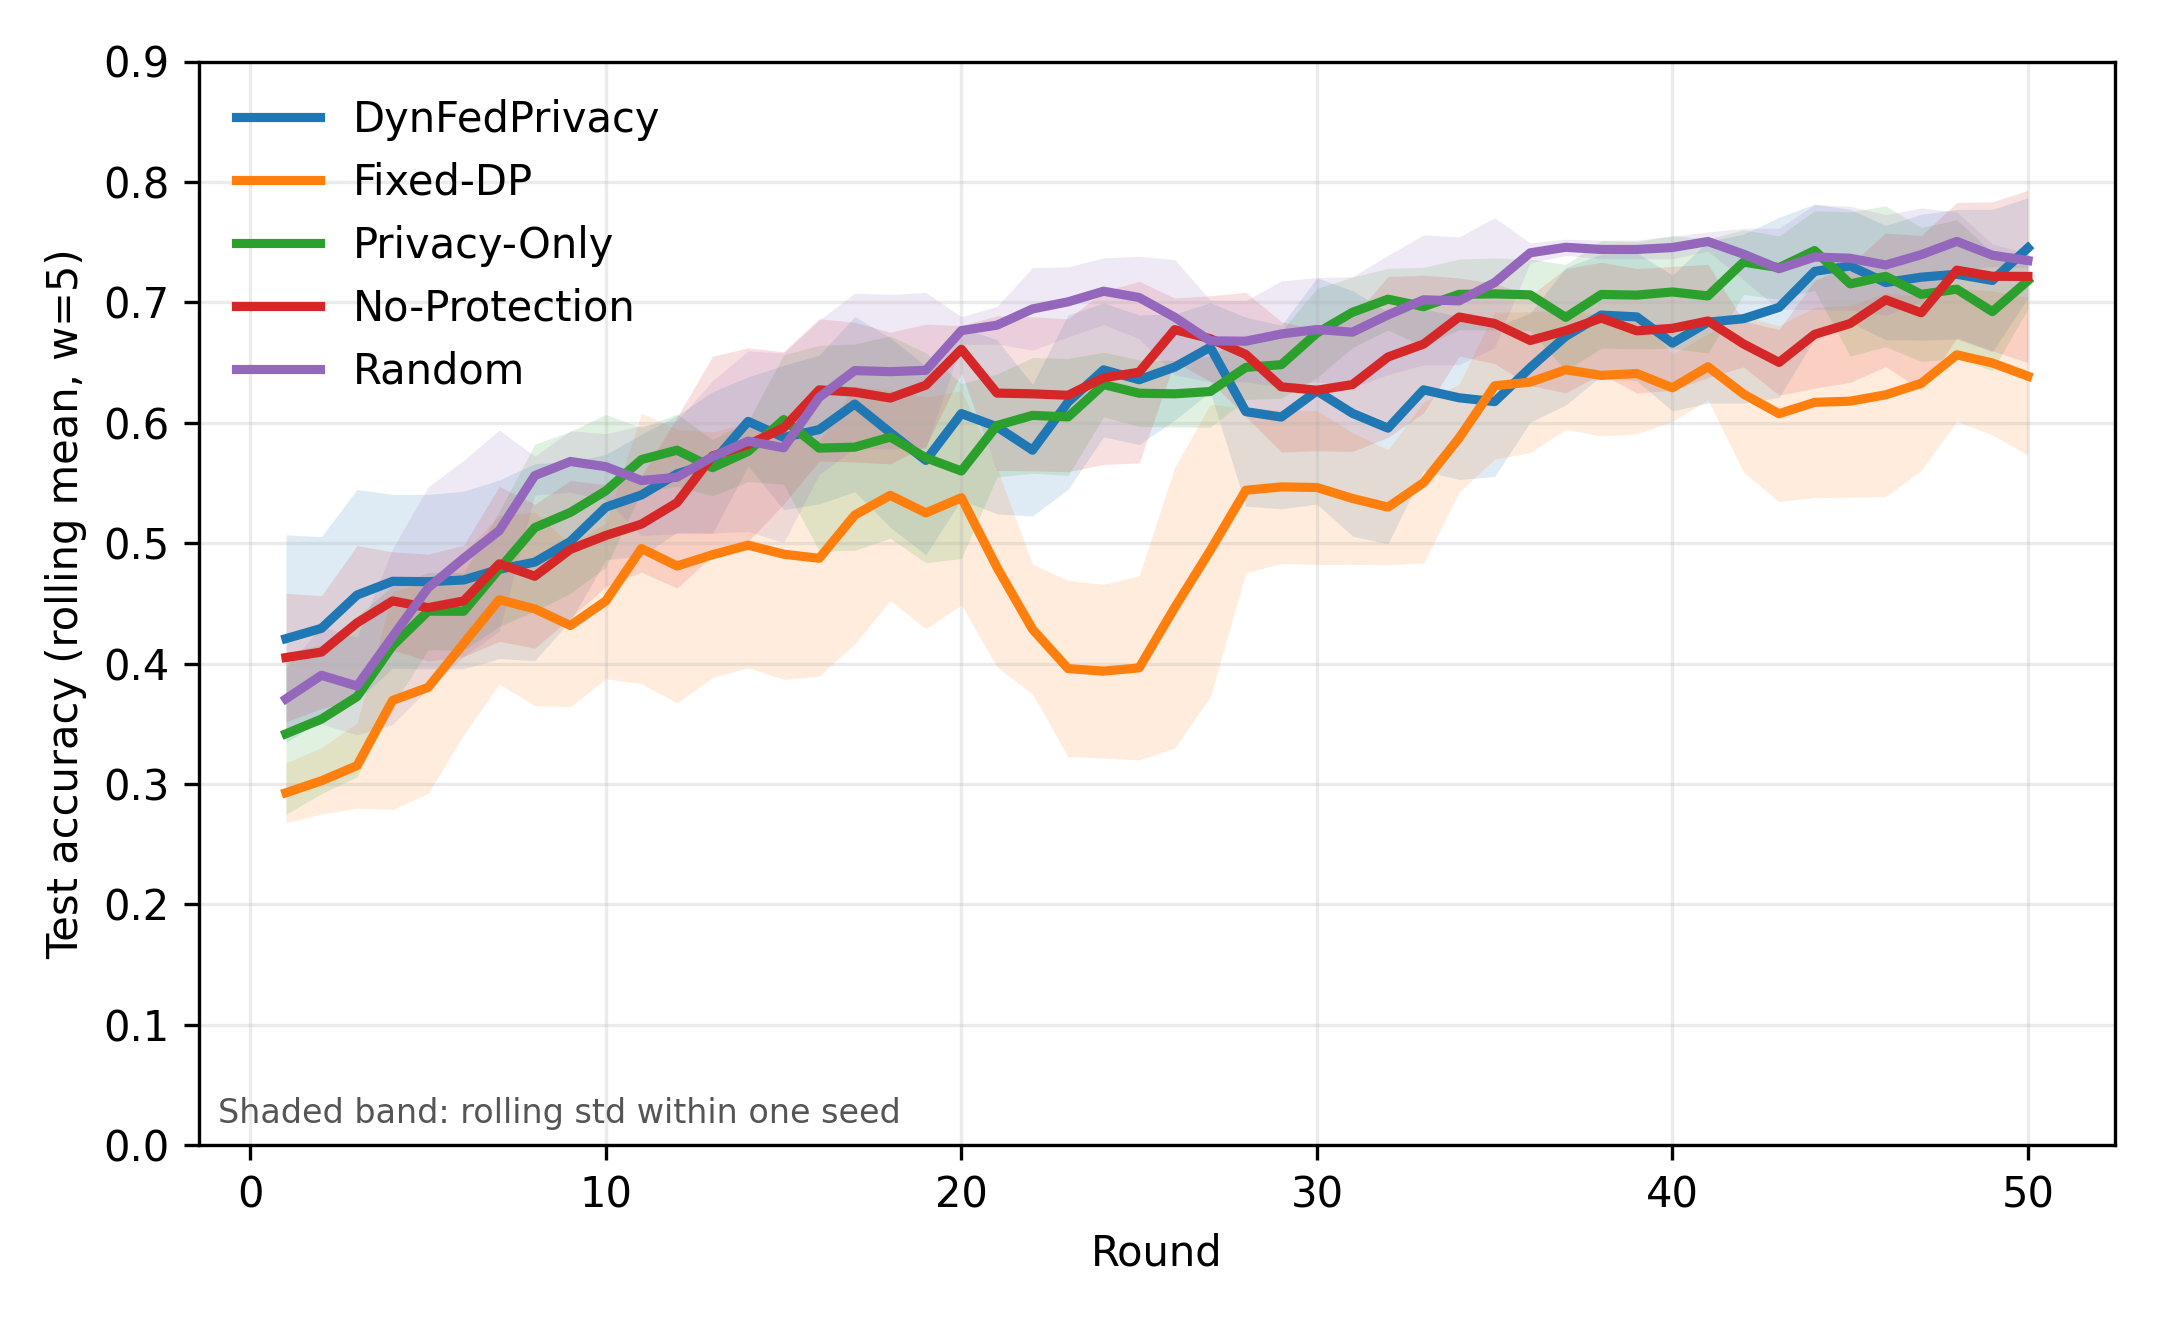
\includegraphics[width=\columnwidth]{fmnist_lenet5_accuracy_convergence_with_random.png}
\caption{Accuracy convergence on Fashion-MNIST with 50 round LeNet-5 real training. Curves are smoothed by a sliding window, and shaded bands represent rolling standard deviation within the same seed.}
\label{fig:accuracy_convergence}
\end{figure}

\begin{figure}[t]
\centering
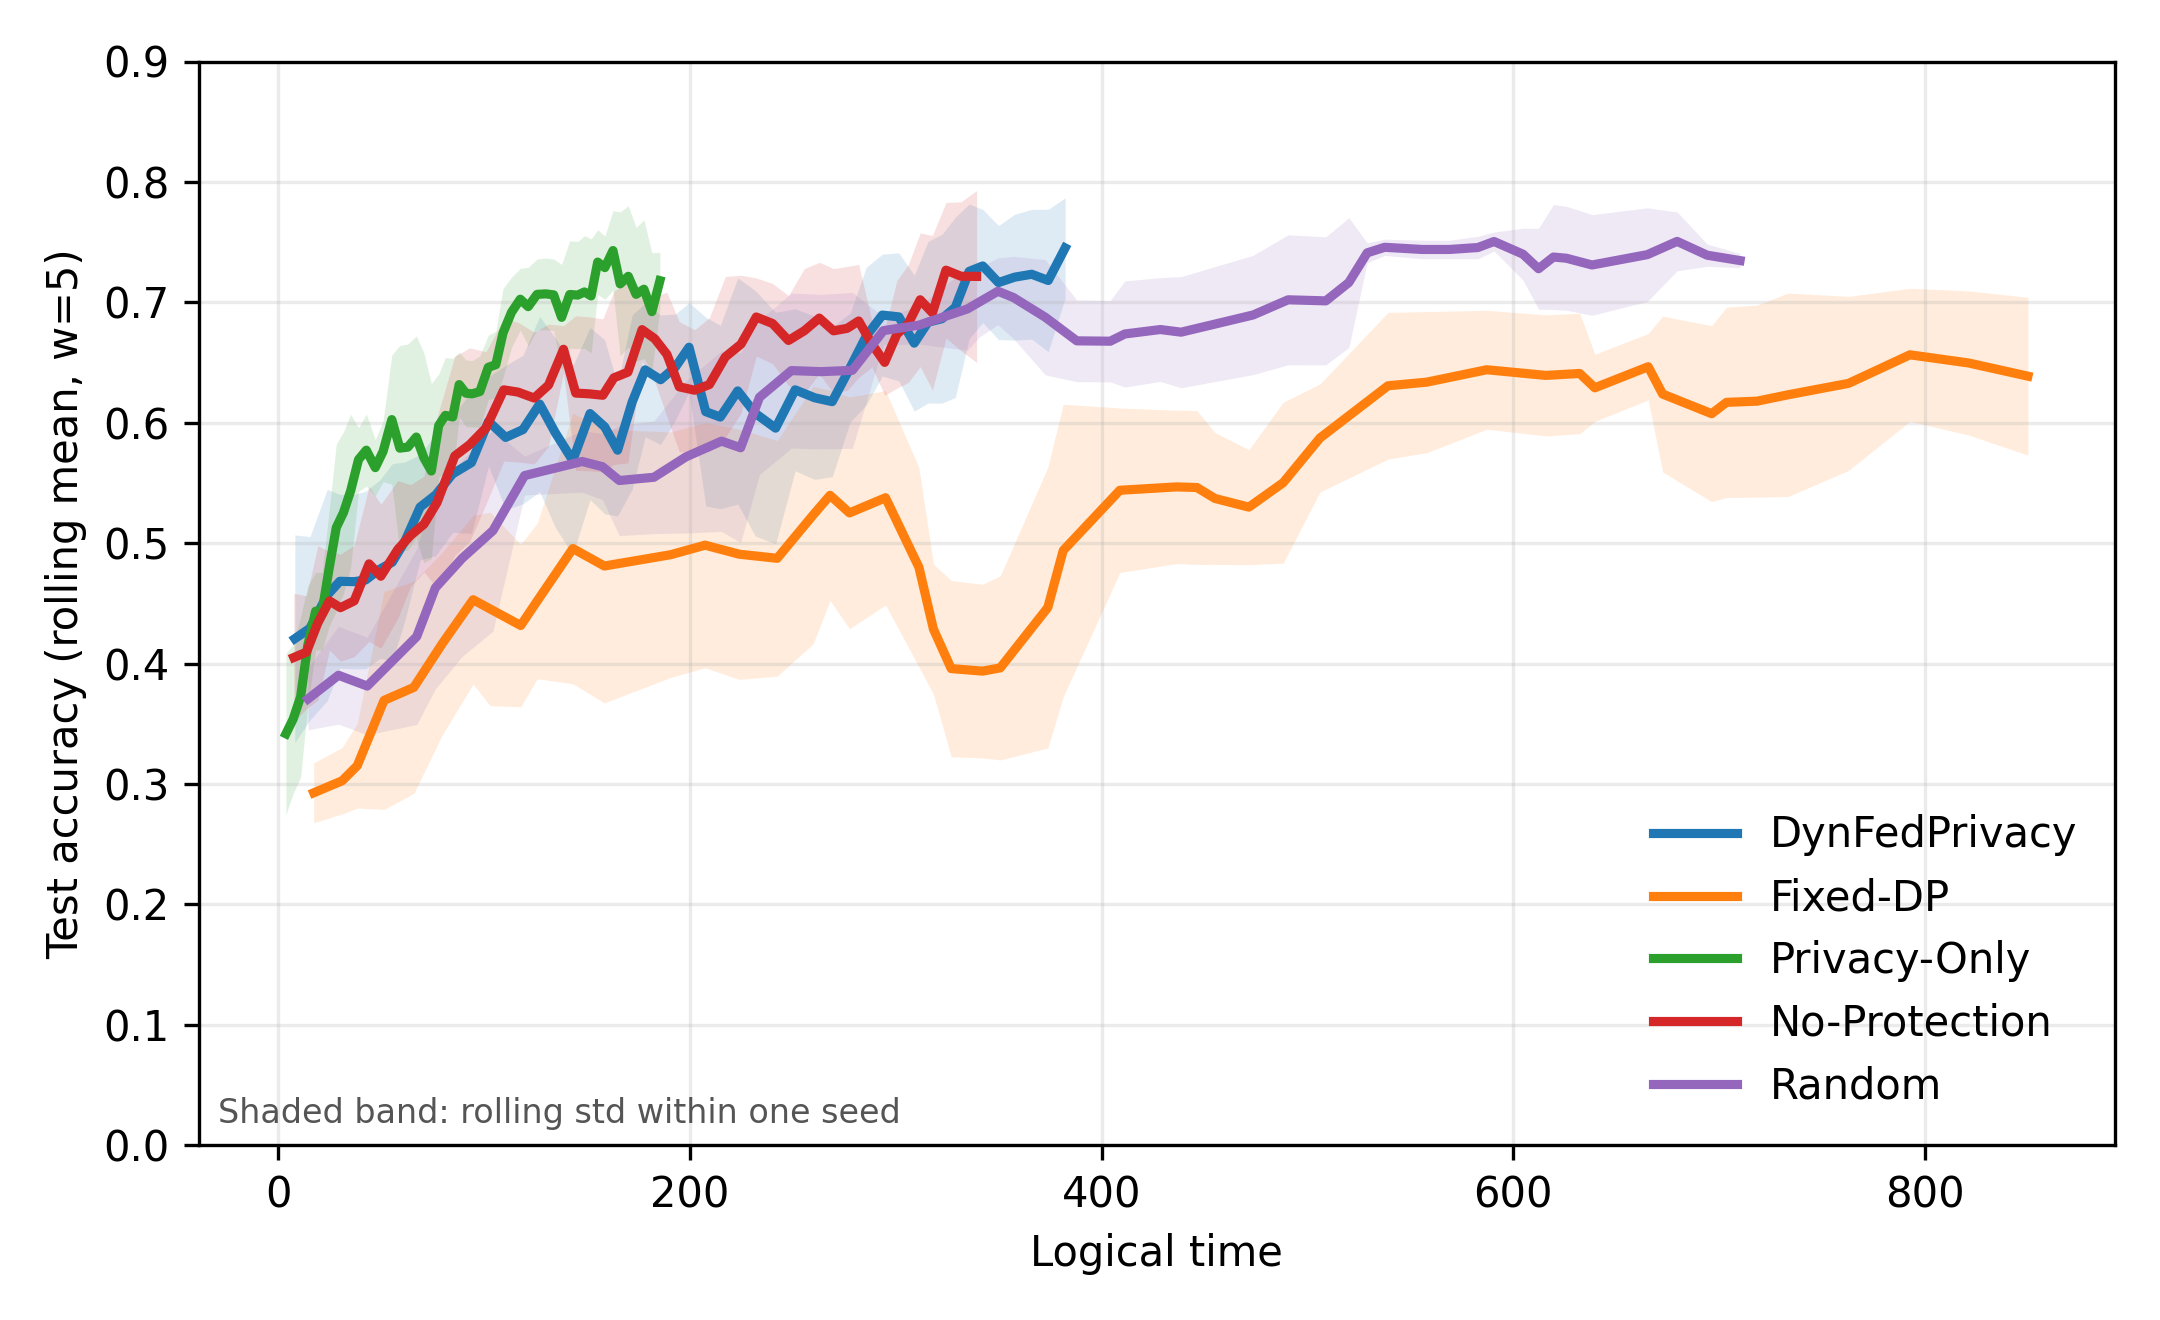
\includegraphics[width=\columnwidth]{fmnist_lenet5_time_accuracy_with_random.png}
\caption{Relationship between logical time and test accuracy in 50 round Fashion-MNIST + LeNet-5 real training.}
\label{fig:time_accuracy}
\end{figure}

\begin{figure}[t]
\centering
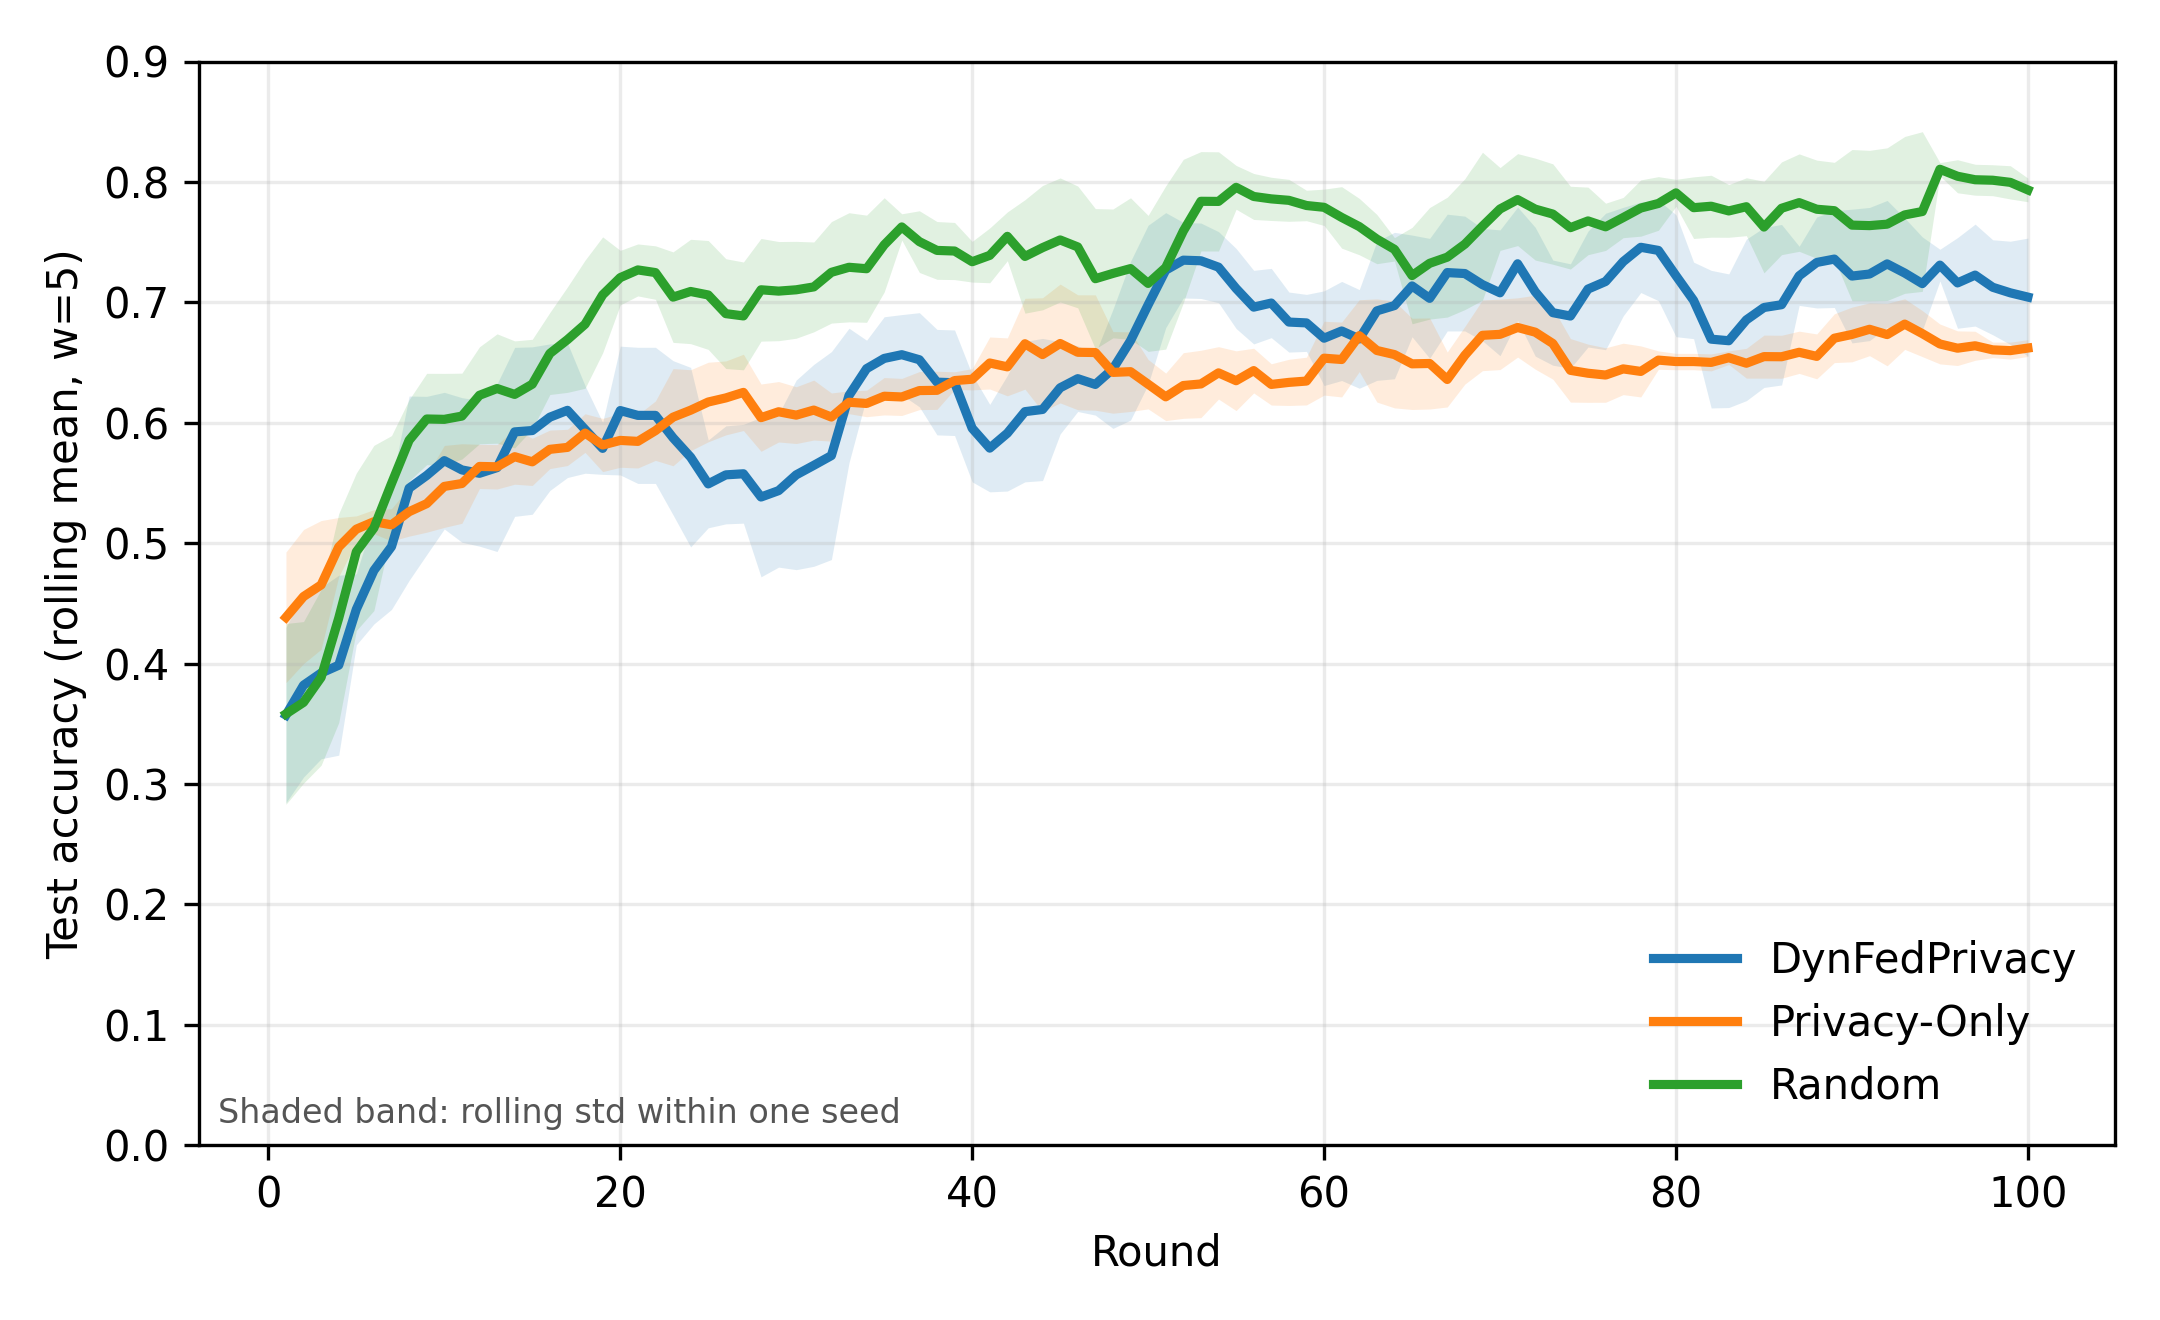
\includegraphics[width=\columnwidth]{fmnist_lenet5_100r_ep3_accuracy.png}
\caption{Accuracy curves for the 100 round, 3 local epoch supplementary Fashion-MNIST + LeNet-5 experiment.}
\label{fig:extension_accuracy}
\end{figure}

\subsection{Dynamic Mode and Privacy Budget Analysis}
\label{sec:mode_privacy}
\figref{fig:mode_distribution} shows the mode distribution of \method{} across device categories.
In 50 round real training, \method{} makes 500 client round decisions.
LIEIIC accounts for 78.4\%, LIIC for 15.8\%, LIIE for 4.8\%, LIC for 0.6\%, LIE for 0.2\%, and LIIEIIIC for 0.2\%.
This result shows that, under the assumption that weak devices can at least execute the encoder side Block and that edge/cloud capacities are reasonably provisioned, the system can find feasible collaborative modes for all devices.
The dominance of LIEIIC and LIIC indicates that decisions are jointly affected by resources, privacy budget, and the global convergence error proxy.
The figure explains mode selection behavior rather than proving that a specific cloud path is inherently more accurate.

\begin{figure}[t]
\centering
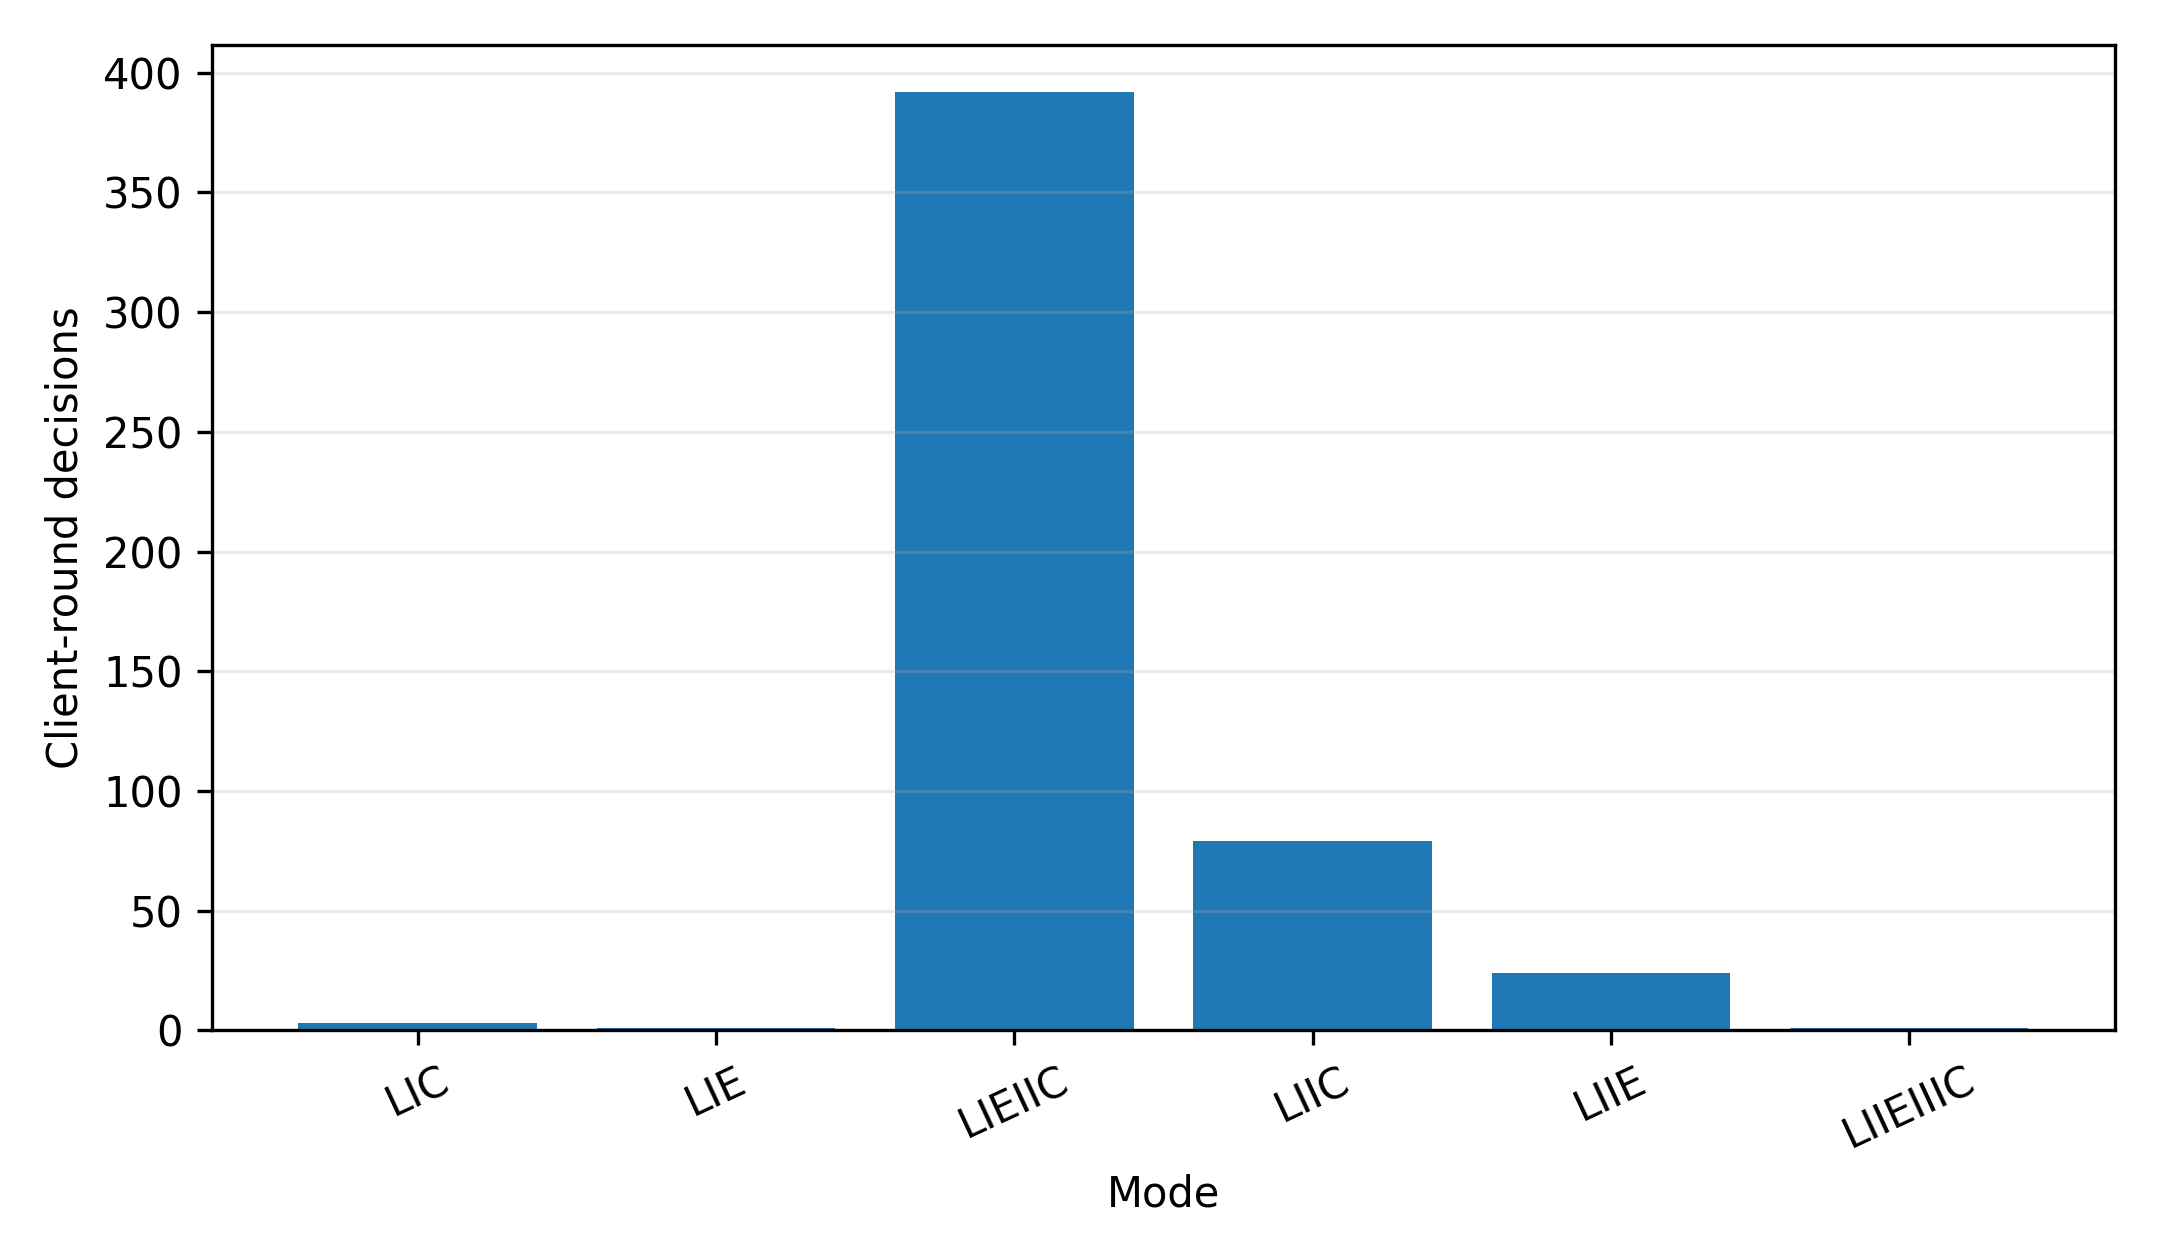
\includegraphics[width=\columnwidth]{fmnist_lenet5_mode_distribution_with_random.png}
\caption{Mode distribution under \method{} across different device categories.}
\label{fig:mode_distribution}
\end{figure}

\figref{fig:privacy_timeline} shows DP budget consumption in real training.
\method{} consumes 23.51 cumulative DP budget, slightly lower than Fixed-DP's 24.22 and higher than Privacy-Only's 10.00.
No-Protection does not enable DP and therefore consumes no DP budget, but it is reported only as a utility reference and is not a protected policy.
These values are cumulative over all devices and rounds, not the remaining budget of one device.
The experiment maintains per device remaining budgets and checks budget feasibility in every round.

\begin{figure}[t]
\centering
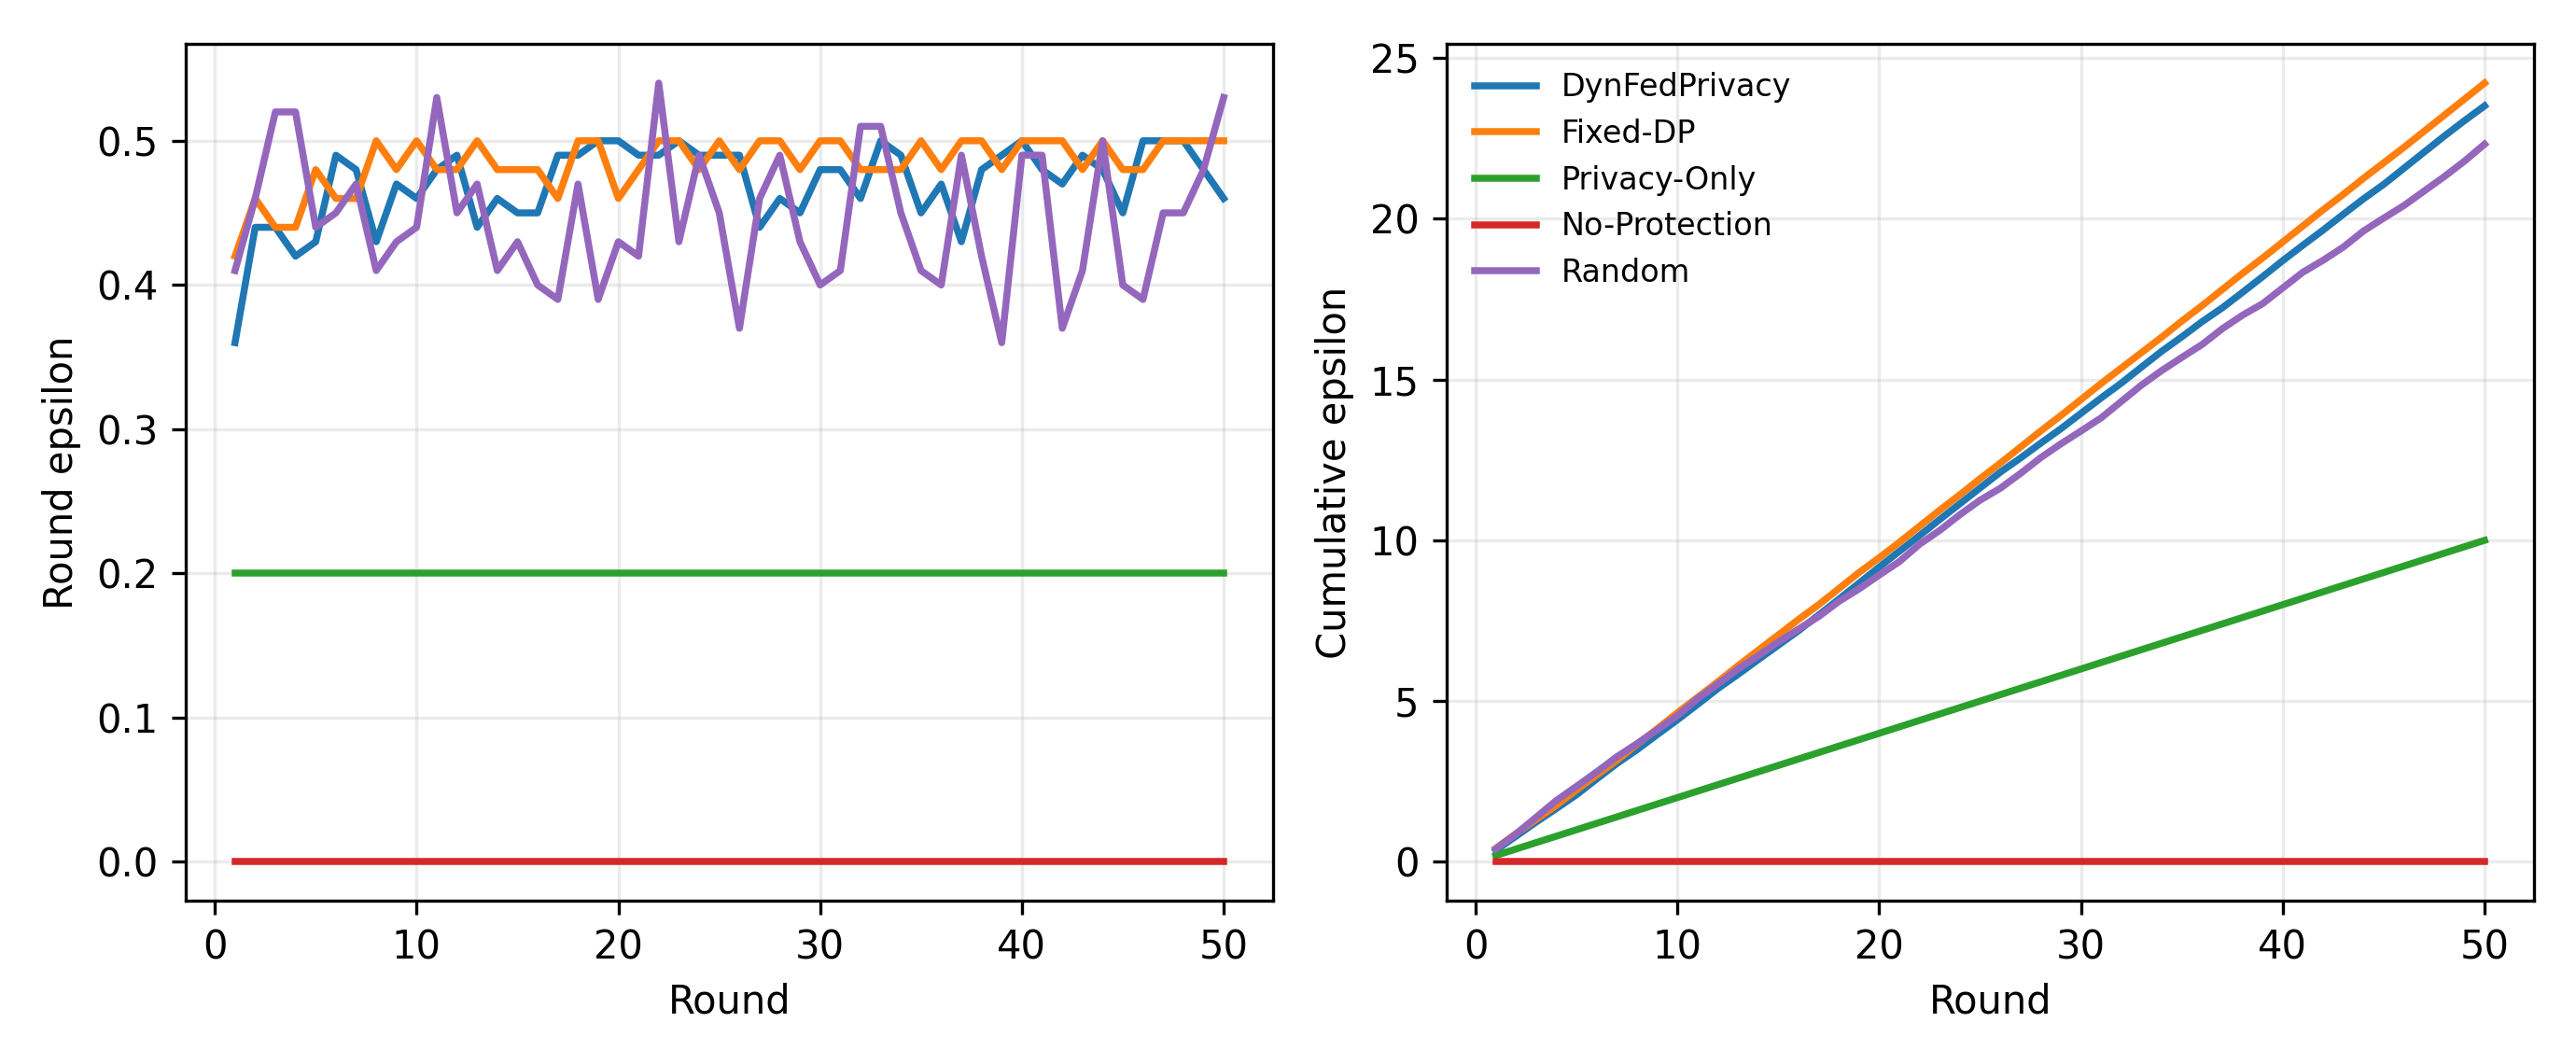
\includegraphics[width=\columnwidth]{fmnist_lenet5_privacy_timeline_with_random.png}
\caption{Privacy budget consumption comparison: per round consumption and cumulative consumption.}
\label{fig:privacy_timeline}
\end{figure}

\subsection{Sensitivity and Robustness Analysis}
\label{sec:ablation}
\textbf{Impact of resource heterogeneity.}
\figref{fig:resource_impact} shows the effect of increasing the weak device ratio \(p_{\mathrm{weak}}\) from 0.2 to 0.8.
\method{} maintains an active ratio of 1.0.
Its latency increases from 1.156 to 1.725, and its global convergence error proxy only increases from 0.120 to 0.148.
This indicates that when weak devices can still execute the encoder side Block, a larger weak device ratio mainly increases training latency but does not cause many devices to be skipped.
\method{} dynamically switches among LIE, LIC, LIEIIC, and LIIE to control the growth of the global convergence error proxy.

\begin{figure}[t]
\centering
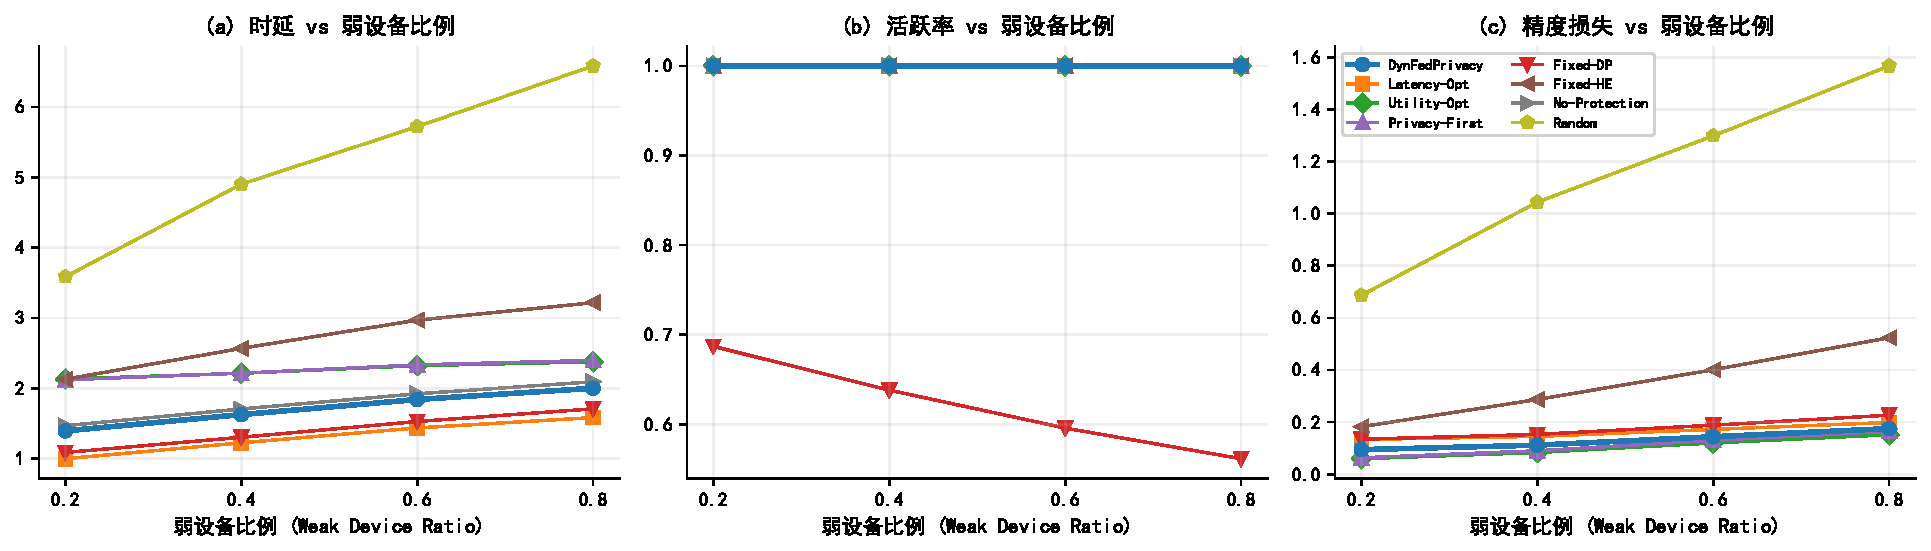
\includegraphics[width=\columnwidth]{fig2_resource_impact.pdf}
\caption{Impact of resource heterogeneity on latency, active ratio, and local convergence error proxy.}
\label{fig:resource_impact}
\end{figure}

\begin{figure}[t]
\centering
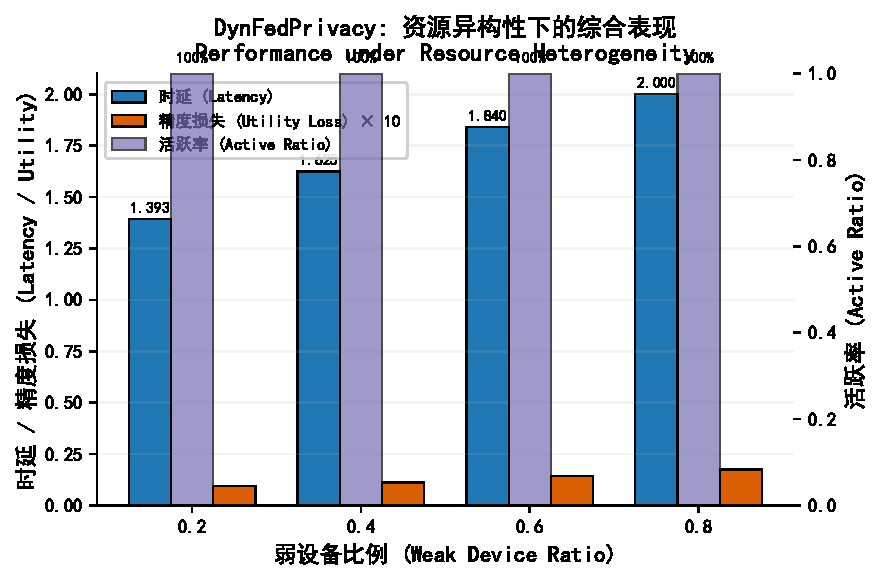
\includegraphics[width=0.60\columnwidth]{fig8_resource_balanced.pdf}
\caption{Detailed behavior of \method{} under resource heterogeneity.}
\label{fig:resource_balanced}
\end{figure}

\textbf{Impact of privacy budget.}
\figref{fig:epsilon_impact} shows the behavior when the initial privacy budget \(\epsilon_0\) varies from 0.5 to 8.0.
\method{} keeps privacy consumption relatively low because its selector judges that excessive DP perturbation can increase the local convergence error proxy under the current DP parameter settings.
Fixed-DP is highly sensitive to \(\epsilon_0\): when \(\epsilon_0\) increases from 0.5 to 4.0, its active ratio rises from 10.6\% to 63.4\%.
This is because under a strict budget, many devices exhaust their DP budgets after only a few rounds.

\begin{figure}[t]
\centering
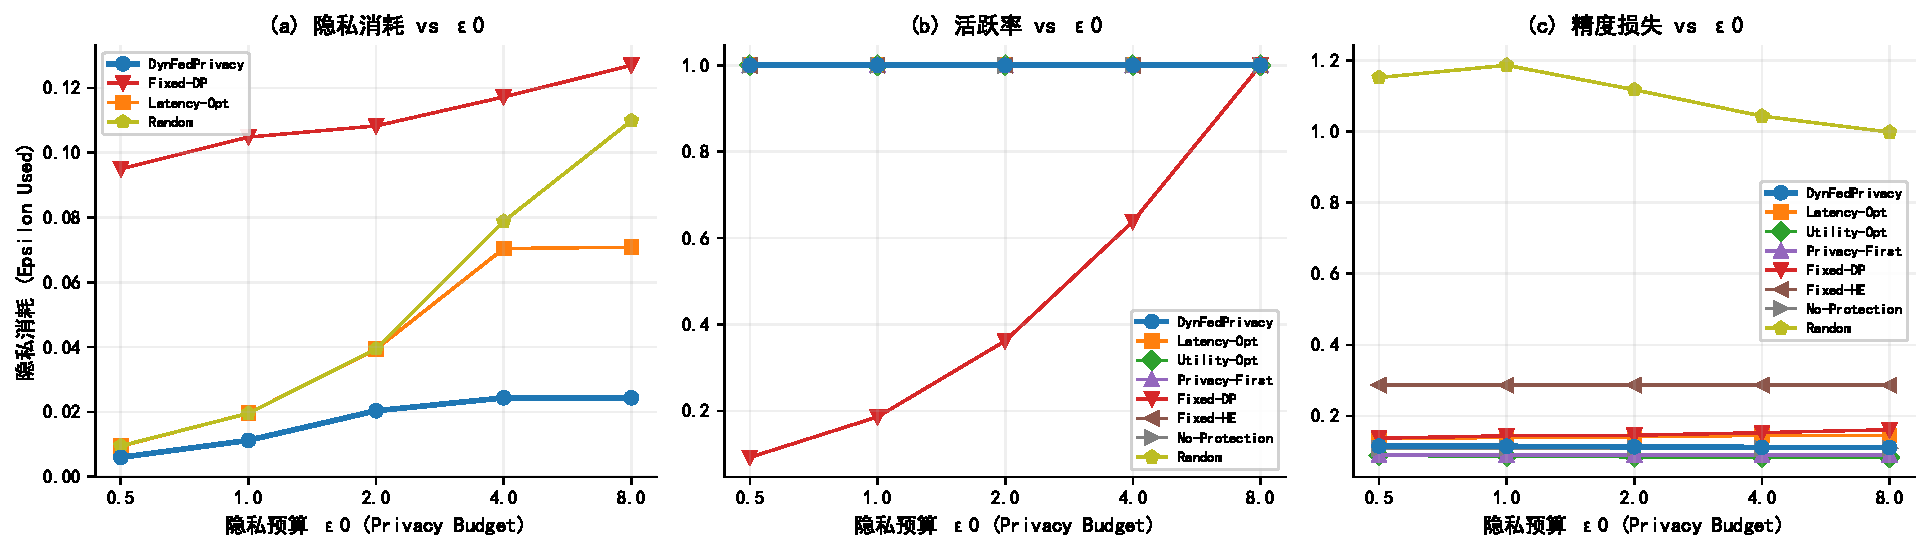
\includegraphics[width=\columnwidth]{fig3_epsilon_impact.pdf}
\caption{Impact of initial privacy budget \(\epsilon_0\) on privacy consumption, active ratio, and local convergence error proxy.}
\label{fig:epsilon_impact}
\end{figure}

\textbf{Impact of network jitter.}
\figref{fig:jitter_impact} shows the impact of the network jitter coefficient.
As jitter increases from 0.0 to 0.75, all policies experience higher latency.
\method's latency increases from 1.338 to 1.424, whereas Fixed-HE increases from 2.177 to 2.539.
The lower growth rate suggests that dynamic mode selection can reduce the impact of network fluctuation on estimated latency under this simulation setting.

\begin{figure}[t]
\centering
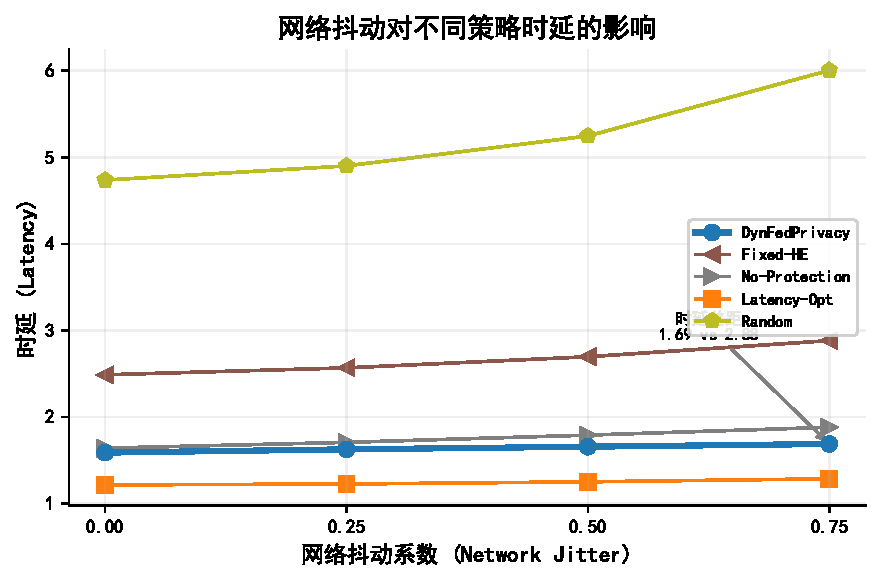
\includegraphics[width=0.55\columnwidth]{fig4_jitter_impact.pdf}
\caption{Impact of network jitter on latency.}
\label{fig:jitter_impact}
\end{figure}

\subsection{CIFAR-10/ResNet-18 Extension for IoTJ Submission}
\label{sec:cifar_results}
We further organize the newer CIFAR-10/ResNet-18 experiments into four ablation groups that directly test the motivation of dynamic hierarchical selection.
Unless otherwise stated, the default configuration is CIFAR-10, pretrained ResNet-18, 200 rounds, seed 42, client heterogeneity 2.0, edge heterogeneity 1.5, SP 1, aggregation fraction 1.0, 3 local epochs, and learning rate \(5\times 10^{-4}\).
The compared methods are \method, Fixed-HFL, Fixed-DP, No-Protection, Individual-Optimal, and Random.
Fixed-HFL corresponds to the fixed LIIEIIIC three layer path.

\textbf{Main comparison across random seeds.}
\tabref{tab:cifar_main} reports the three seed result under extreme edge label skew.
\method{} obtains the highest mean best accuracy among non random structured policies and reduces logical time by 24.2\% compared with Fixed-HFL.
Random reaches a high best accuracy in some runs, but its logical time is much larger and the selected modes are unconstrained.
This supports the central claim that the proposed dynamic hierarchy improves the efficiency utility tradeoff rather than simply overfitting to one seed.

\begin{table*}[t]
\centering
\caption{CIFAR-10/ResNet-18 Main Comparison Across Three Random Seeds Under Extreme Edge Label Skew}
\label{tab:cifar_main}
\begin{tabular}{lccccc}
\hline
\textbf{Policy} & \textbf{Final Acc.} & \textbf{Best Acc.} & \textbf{Avg. Last 10 Acc.} & \textbf{Logical Time} & \textbf{Skip Rate} \\
\hline
\method{} & \(0.578\pm0.021\) & \(0.622\pm0.003\) & \(0.587\pm0.014\) & 2767.5 & 0.000 \\
Fixed-HFL & \(0.564\pm0.027\) & \(0.599\pm0.007\) & \(0.564\pm0.027\) & 3652.7 & 0.170 \\
Fixed-DP & \(0.557\pm0.044\) & \(0.597\pm0.000\) & \(0.563\pm0.019\) & 7193.8 & 0.000 \\
No-Protection & \(0.563\pm0.020\) & \(0.608\pm0.002\) & \(0.572\pm0.004\) & 7047.4 & 0.000 \\
Individual-Optimal & \(0.587\pm0.010\) & \(0.620\pm0.011\) & \(0.578\pm0.019\) & 2716.6 & 0.000 \\
Random & \(0.551\pm0.023\) & \(0.640\pm0.008\) & \(0.560\pm0.011\) & 6107.8 & 0.000 \\
\hline
\end{tabular}
\end{table*}

\begin{figure*}[t]
\centering
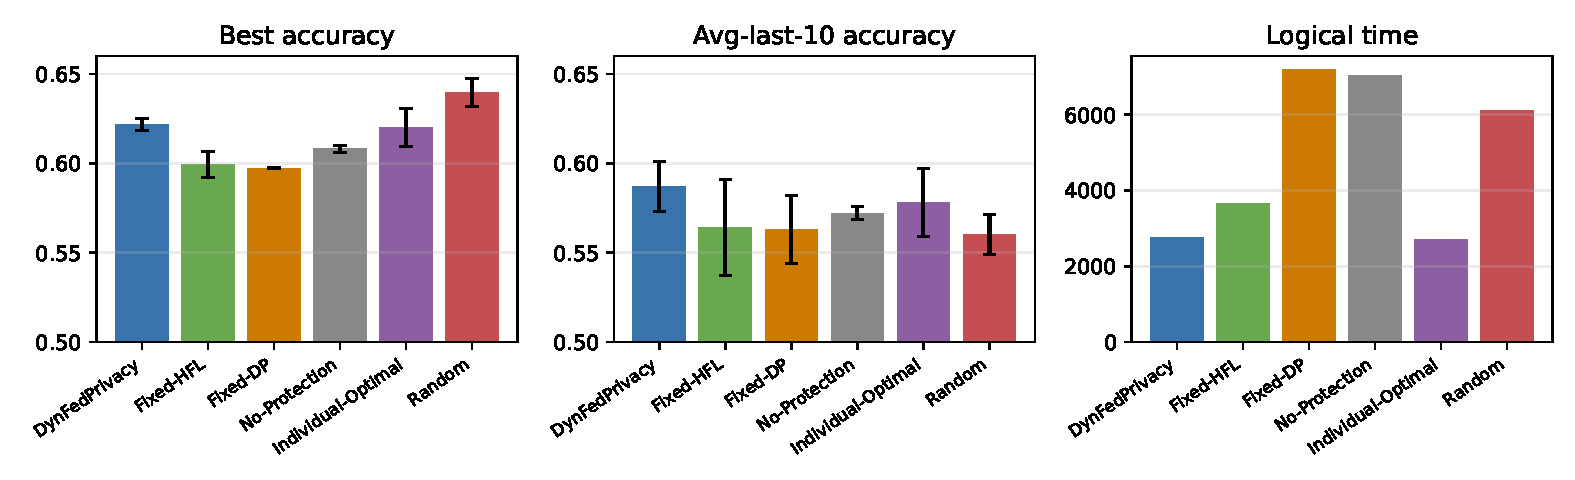
\includegraphics[width=0.95\textwidth]{main_multiseed_summary.pdf}
\caption{CIFAR-10/ResNet-18 summary across three random seeds: best accuracy, average last 10 accuracy, and logical time.}
\label{fig:main_multiseed_summary}
\end{figure*}

\textbf{Data distribution ablation.}
The highest priority ablation evaluates whether the advantage of dynamic hierarchy comes from non-IID and edge level heterogeneity rather than an accidental random seed.
\tabref{tab:data_distribution_ablation} and \figref{fig:data_distribution_ablation} compare IID, client non-IID, edge label skew, and extreme edge label skew using the fixed seed 42 setting.
Under IID data, all structured policies obtain similar best accuracy, and the main difference is efficiency.
As the data distribution becomes more heterogeneous, \method{} becomes more favorable relative to Fixed-HFL: under client non-IID, \method{} improves best accuracy from 0.604 to 0.620 while reducing logical time from 3609.6 to 2758.5; under edge label skew, it improves best accuracy from 0.647 to 0.666 while reducing logical time from 3625.5 to 2707.1.
Under extreme edge label skew, \method{} improves best accuracy from 0.592 to 0.622 and reduces logical time from 3625.5 to 2701.6.
These results indicate that dynamic hierarchical selection is most useful when cross client and cross edge data heterogeneity makes a fixed path inefficient.

\begin{table*}[t]
\centering
\caption{Data Distribution Ablation on CIFAR-10/ResNet-18}
\label{tab:data_distribution_ablation}
\begin{tabular}{llcccc}
\hline
\textbf{Distribution} & \textbf{Policy} & \textbf{Best Acc.} & \textbf{Avg. Last 10 Acc.} & \textbf{Logical Time} & \textbf{Comm.} \\
\hline
\multirow{6}{*}{IID}
 & \method{} & 0.730 & 0.726 & 2750.5 & 38612.4 \\
 & Fixed-HFL & 0.730 & 0.729 & 3624.4 & 16932.0 \\
 & Fixed-DP & 0.736 & 0.731 & 7193.5 & 44641.7 \\
 & No-Protection & 0.731 & 0.722 & 7052.5 & 43756.4 \\
 & Individual-Optimal & 0.730 & 0.726 & 2678.2 & 41895.2 \\
 & Random & 0.744 & 0.734 & 6160.0 & 33111.2 \\
\midrule
\multirow{6}{*}{Client non-IID}
 & \method{} & 0.620 & 0.600 & 2758.5 & 38612.4 \\
 & Fixed-HFL & 0.604 & 0.568 & 3609.6 & 16932.0 \\
 & Fixed-DP & 0.608 & 0.570 & 7201.7 & 44641.7 \\
 & No-Protection & 0.617 & 0.597 & 7055.3 & 43756.4 \\
 & Individual-Optimal & 0.643 & 0.611 & 2695.0 & 41895.2 \\
 & Random & 0.673 & 0.608 & 6147.3 & 33111.2 \\
\midrule
\multirow{6}{*}{Edge label skew}
 & \method{} & 0.666 & 0.614 & 2707.1 & 37258.6 \\
 & Fixed-HFL & 0.647 & 0.587 & 3625.5 & 16932.0 \\
 & Fixed-DP & 0.638 & 0.593 & 7202.2 & 44641.7 \\
 & No-Protection & 0.664 & 0.600 & 7054.4 & 43756.4 \\
 & Individual-Optimal & 0.674 & 0.602 & 2697.1 & 41895.2 \\
 & Random & 0.693 & 0.624 & 6160.2 & 33111.2 \\
\midrule
\multirow{6}{*}{Extreme edge skew}
 & \method{} & 0.622 & 0.602 & 2701.6 & 37853.6 \\
 & Fixed-HFL & 0.592 & 0.585 & 3625.5 & 16932.0 \\
 & Fixed-DP & 0.598 & 0.563 & 7229.0 & 45379.0 \\
 & No-Protection & 0.608 & 0.569 & 7064.7 & 44439.6 \\
 & Individual-Optimal & 0.619 & 0.577 & 2678.2 & 42740.4 \\
 & Random & 0.631 & 0.564 & 6146.1 & 33111.2 \\
\hline
\end{tabular}
\end{table*}

\begin{figure*}[t]
\centering
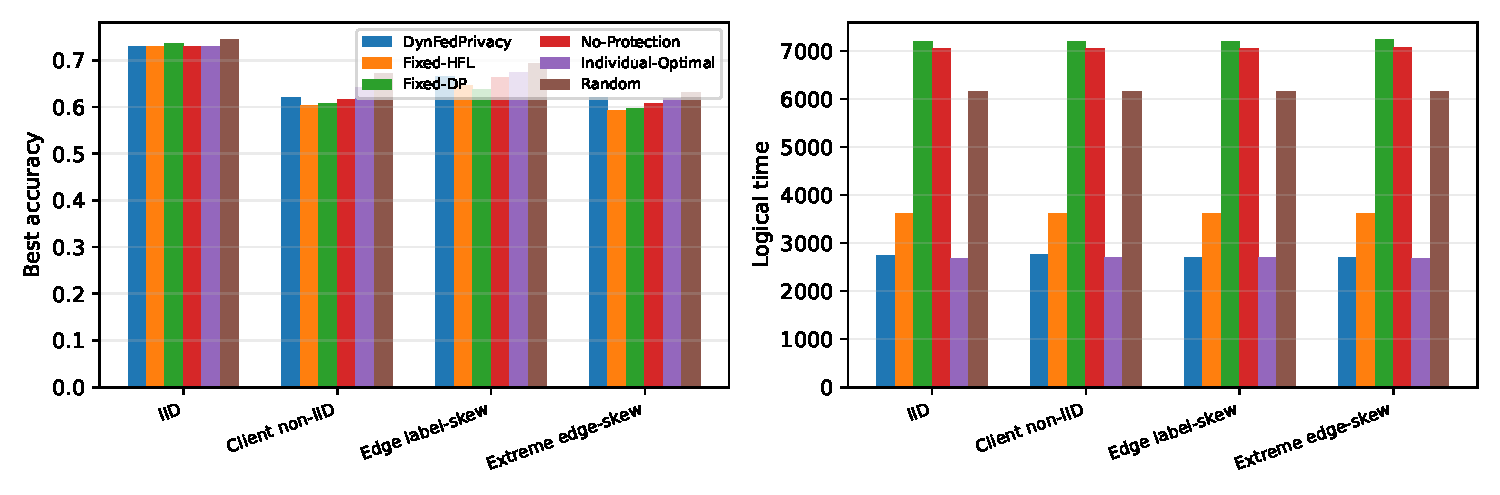
\includegraphics[width=0.95\textwidth]{data_distribution_ablation.pdf}
\caption{CIFAR-10/ResNet-18 data distribution ablation.}
\label{fig:data_distribution_ablation}
\end{figure*}

\textbf{Resource heterogeneity ablation.}
The second high priority ablation evaluates whether \method{} is suitable for heterogeneous cloud-edge-end systems.
We fix the data distribution to extreme edge label skew and compare client/edge heterogeneity levels 1.0/1.0, 2.0/1.5, and 4.0/3.0.
\tabref{tab:resource_heterogeneity_ablation} summarizes \method's detailed behavior.
The feasible rate remains 1.0 and the skip rate remains 0 across all three settings, while Fixed-HFL has a persistent 0.17 skip rate because the fixed LIIEIIIC path cannot effectively absorb all delayed clients.
As heterogeneity increases to 4.0/3.0, Fixed-HFL's logical time rises to 4211.8, whereas \method{} remains at 2732.9.
The mode distribution also changes: \method{} reduces the share of LIEIIC from 0.66 to 0.57 and increases LIIC to 0.38 under stronger heterogeneity, indicating that it actively reallocates computation and aggregation paths.

\begin{table*}[t]
\centering
\caption{Resource Heterogeneity Ablation of \method{} Under Extreme Edge Label Skew}
\label{tab:resource_heterogeneity_ablation}
\begin{tabular}{lcccccl}
\hline
\textbf{Client/Edge Het.} & \textbf{Best Acc.} & \textbf{Avg. Last 10} & \textbf{Logical Time} & \textbf{Feasible Rate} & \textbf{Skip Rate} & \textbf{Dominant Modes} \\
\hline
1.0/1.0 & 0.623 & 0.596 & 2756.3 & 1.000 & 0.000 & LIEIIC 0.65, LIIC 0.28 \\
2.0/1.5 & 0.622 & 0.602 & 2701.6 & 1.000 & 0.000 & LIEIIC 0.66, LIIC 0.30 \\
4.0/3.0 & 0.638 & 0.566 & 2732.9 & 1.000 & 0.000 & LIEIIC 0.57, LIIC 0.38 \\
\hline
\end{tabular}
\end{table*}

\begin{figure*}[t]
\centering
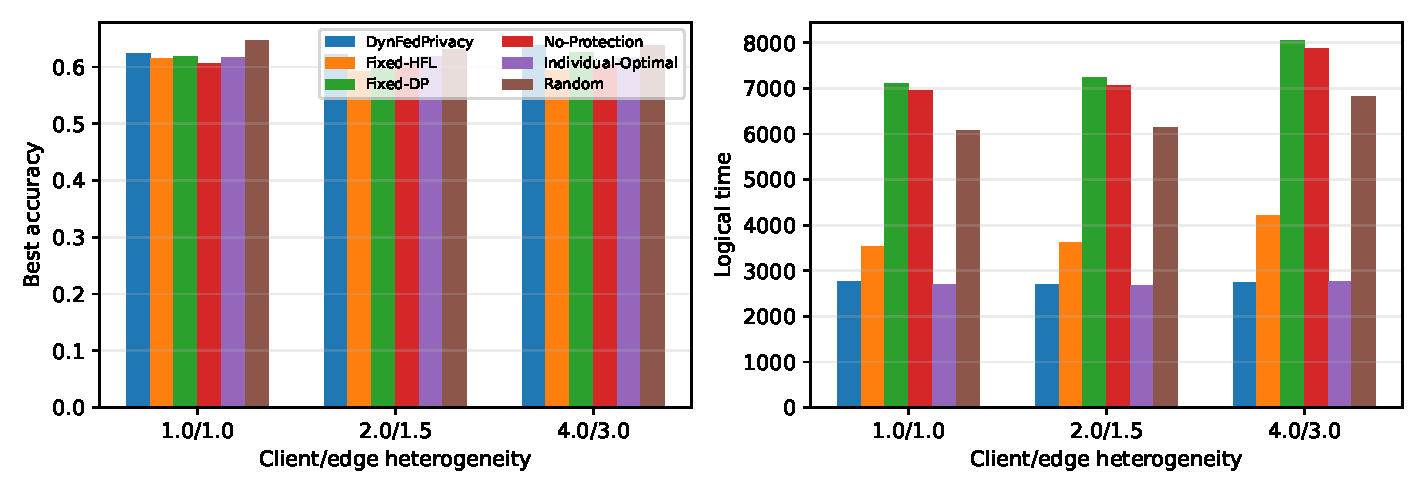
\includegraphics[width=0.95\textwidth]{resource_heterogeneity_ablation.pdf}
\caption{CIFAR-10/ResNet-18 resource heterogeneity ablation.}
\label{fig:resource_heterogeneity_fig}
\end{figure*}

\textbf{Strategy update period ablation.}
The SP ablation studies how frequently the system should reconfigure hierarchical modes.
\added[id=R1]{This experiment is motivated by switching-cost-aware FL methods, where changing the selected participants every round can incur non-negligible reconfiguration overhead and block-wise updates are used to reduce cumulative switching costs~\cite{CHEN2026112204,10757319}. In our setting, a small \(S_P\) allows faster adaptation to resource, privacy, and link changes, whereas a large \(S_P\) keeps hierarchical modes stable for longer intervals and reduces potential model-block migration, state synchronization, and scheduling reconfiguration.}
We run only \method{} under extreme edge label skew with client/edge heterogeneity 4.0/3.0 and vary SP from 1 to 20.
\tabref{tab:sp_sensitivity} and \figref{fig:sp_sensitivity} show that SP=5 gives the highest final and average last 10 accuracy among the tested periods, while SP=1 gives the highest best accuracy.
Increasing SP reduces communication slightly but delays adaptation to resource and link changes.
Thus, frequent reconfiguration is useful under strong heterogeneity, but a moderate period can stabilize late round behavior.
\added[id=R1]{Therefore, the SP results should be interpreted as an adaptation-stability tradeoff: per-round updates provide the most responsive policy, while moderate block-wise updates reduce unnecessary reconfiguration without fully losing adaptivity. The current simulation does not directly measure real deployment costs such as optimizer-state migration or cryptographic-context setup, so explicit measurement of \(C_i^{\mathrm{sw},t}\) remains an important deployment-oriented extension.}

\begin{table*}[t]
\centering
\caption{Strategy Update Period Ablation for \method}
\label{tab:sp_sensitivity}
\begin{tabular}{lccccccl}
\hline
\textbf{SP} & \textbf{Best Acc.} & \textbf{Avg. Last 10} & \textbf{Logical Time} & \textbf{Comm.} & \textbf{Feasible Rate} & \textbf{Skip Rate} & \textbf{Dominant Modes} \\
\hline
1 & 0.638 & 0.566 & 2732.9 & 35601.5 & 1.000 & 0.000 & LIEIIC 0.57, LIIC 0.38 \\
5 & 0.624 & 0.592 & 2735.5 & 35549.1 & 1.000 & 0.000 & LIEIIC 0.57, LIIC 0.38 \\
10 & 0.609 & 0.576 & 2780.4 & 35326.4 & 1.000 & 0.000 & LIEIIC 0.56, LIIC 0.38 \\
20 & 0.618 & 0.580 & 2866.1 & 34371.3 & 1.000 & 0.000 & LIEIIC 0.52, LIIC 0.39 \\
\hline
\end{tabular}
\end{table*}

\begin{figure}[t]
\centering
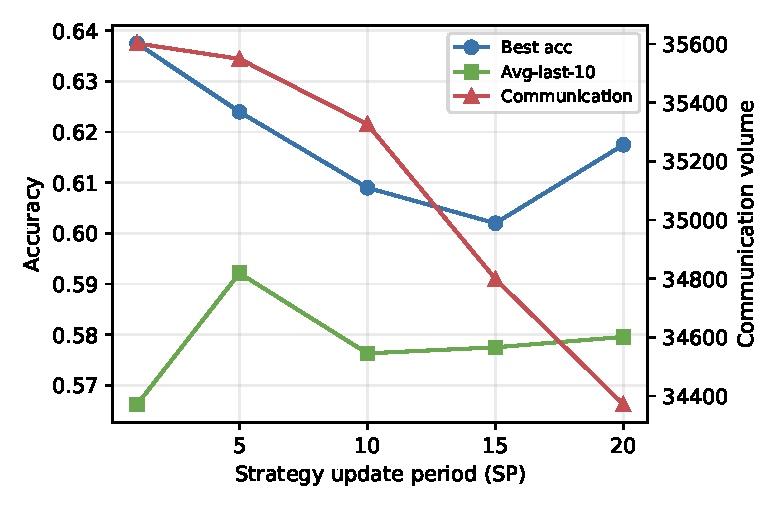
\includegraphics[width=\columnwidth]{sp_sensitivity.pdf}
\caption{Sensitivity to strategy update period in the CIFAR-10/ResNet-18 experiment.}
\label{fig:sp_sensitivity}
\end{figure}

\textbf{Aggregation fraction ablation.}
The aggregation fraction ablation explains how the asynchronous aggregation ratio affects efficiency and accuracy fluctuation.
We compare \method{} and Fixed-HFL at aggregation fractions 0.5, 0.7, and 1.0.
\tabref{tab:aggregation_fraction_ablation} shows that partial aggregation reduces logical time, but an overly small fraction may lower average last 10 accuracy because fewer updates participate in each aggregation event.
At aggregation fraction 0.5, \method{} improves best accuracy over Fixed-HFL from 0.505 to 0.611 and reduces logical time from 2880.4 to 2087.1.
At aggregation fraction 0.7, \method{} improves best accuracy from 0.567 to 0.624 and reduces logical time from 3514.9 to 2665.7.
At aggregation fraction 1.0, \method{} improves best accuracy from 0.592 to 0.622 and reduces logical time from 3625.5 to 2701.6.

\begin{table*}[t]
\centering
\caption{Aggregation Fraction Ablation on CIFAR-10/ResNet-18}
\label{tab:aggregation_fraction_ablation}
\begin{tabular}{lccccc}
\hline
\textbf{Agg. Fraction} & \textbf{Policy} & \textbf{Local Epochs} & \textbf{Best Acc.} & \textbf{Avg. Last 10} & \textbf{Logical Time} \\
\hline
0.5 & \method{} & 3 & 0.611 & 0.520 & 2087.1 \\
0.5 & Fixed-HFL & 3 & 0.505 & 0.407 & 2880.4 \\
0.7 & \method{} & 3 & 0.624 & 0.577 & 2665.7 \\
0.7 & Fixed-HFL & 3 & 0.567 & 0.527 & 3514.9 \\
1.0 & \method{} & 3 & 0.622 & 0.602 & 2701.6 \\
1.0 & Fixed-HFL & 3 & 0.592 & 0.585 & 3625.5 \\
\hline
\end{tabular}
\end{table*}

\begin{figure}[t]
\centering
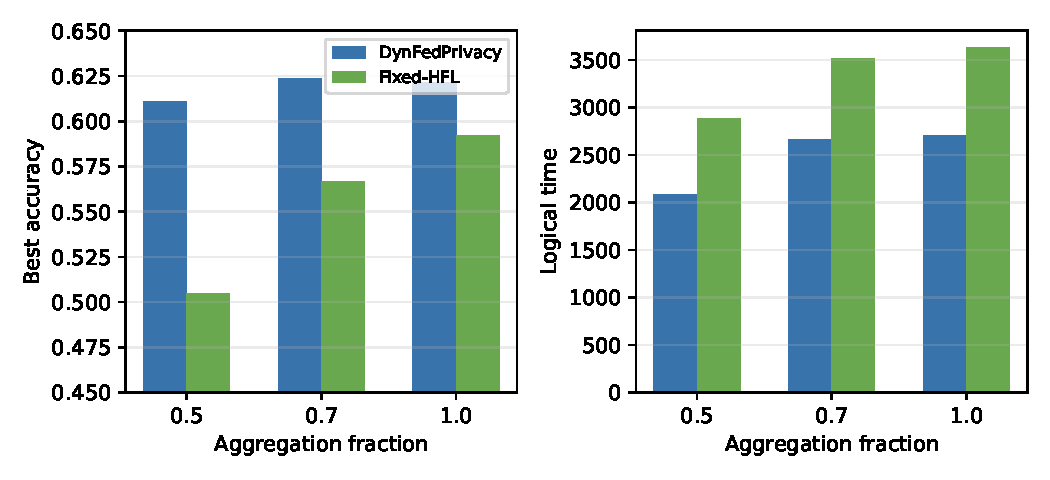
\includegraphics[width=\columnwidth]{aggregation_fraction_ablation.pdf}
\caption{Aggregation fraction ablation in the CIFAR-10/ResNet-18 experiment.}
\label{fig:aggregation_fraction_ablation}
\end{figure}

\subsection{Discussion}
\label{sec:discussion}
Overall, the experiments support three observations.
First, dynamic hierarchical selection can maintain resource feasibility and adapt computation placement under heterogeneous devices.
Second, privacy mechanisms should not be imposed uniformly on all transmissions.
Fixed-DP may increase latency or exhaust privacy budgets, while HE should be treated as a high cost encrypted transmission option unless a real cryptographic implementation is used.
Third, test accuracy and the convergence error proxy should be separated.
The selector optimizes latency and a system level proxy, while test accuracy evaluates the empirical effect of the resulting training behavior.
The Fashion-MNIST results show the limits of the current weight setting, and the CIFAR-10/ResNet-18 extension indicates that dynamic selection can improve the cost utility tradeoff under stronger heterogeneity and longer training.

\section{Conclusion}
\label{sec:conclusion}
This paper studied hierarchical mode selection for cloud-edge-end federated learning under resource constraints and privacy protection.
We constructed resource feasible mode sets for heterogeneous end devices, defined a Block and Flow representation for cloud-edge-end collaborative links, modeled latency, DP budget consumption, and DP induced convergence error effects, and proposed an ideal point based dynamic mode selection algorithm.

In system simulation, \method{} maintains an active ratio of 1.0 and obtains a cloud fusion ratio of 0.456 under the default setting, showing that weak devices can avoid being skipped through hierarchical mode selection.
In 50 round Fashion-MNIST + LeNet-5 real training, \method{} reaches 63.25\% final accuracy and 72.80\% best accuracy, while reducing logical time from 819.59 to 355.20 compared with Fixed-DP.
The 100 round, 3 local epoch supplementary experiment further shows that \method{} improves final and best accuracy over Privacy-Only.
The CIFAR-10/ResNet-18 extension shows that, under extreme edge label skew across three seeds, \method{} improves average best accuracy over Fixed-HFL from 0.5992 to 0.6217 and reduces logical time from 3652.7 to 2767.5.
These results indicate that the proposed framework provides a tunable privacy utility efficiency tradeoff, while further weight search, multiple seed real training, and additional datasets are still needed for a stronger submission.

\appendix
\section{Interpretation of the HE Overhead Model}
\label{app:he_model}
HE is included as a candidate privacy mechanism through a system level overhead model.
For a transmitted object of size \(S\), the effective size under HE is modeled as \(\alpha_{\mathrm{HE}}S\), where \(\alpha_{\mathrm{HE}}>1\) represents ciphertext encoding and packing expansion.
An additional processing latency \(T^P(\mathrm{HE})\) is also added to the communication path.
This abstraction is useful for evaluating whether a dynamic selector avoids high cost encrypted paths when they are not beneficial.
It is not an implementation of CKKS, BFV, or another real HE cryptosystem.
Therefore, all HE related conclusions should be interpreted as system level overhead analysis rather than end to end encrypted training performance.

\section{Baseline Semantics}
\label{app:baselines}
Fixed-DP isolates the effect of applying the same DP mechanism to all eligible transmissions.
Fixed-HE isolates the effect of high cost encrypted update transmission.
Fixed-HFL in the CIFAR-10 experiments forces clients to use the LIIEIIIC three layer path.
Privacy-Only prioritizes low privacy risk and illustrates the gap between privacy preference alone and multi objective optimization.
No-Protection provides a utility reference without DP perturbation and should not be treated as privacy preserving.
Individual-Optimal selects locally strong decisions and illustrates the gap between local utility and system level tradeoff.
Random represents unconstrained path exploration; its high instantaneous accuracy in some settings does not imply stable or cost efficient training.
\bibliographystyle{elsarticle-num}
\bibliography{refs}

\end{document}
